%\documentclass[manuscript]{biometrika}
\documentclass[lineno]{biometrika}

\usepackage{amsmath}
%\usepackage{varwidth}

%% Please use the following statements for
%% managing the text and math fonts for your papers:
\usepackage{times}
\usepackage{bm}
\usepackage{natbib}

\makeatletter

\usepackage{verbatim}
\usepackage{graphicx,epsfig}
\usepackage{amsmath,amssymb,latexsym, amsfonts, amscd}

\usepackage[plain,noend]{algorithm2e}

\makeatletter
\renewcommand{\algocf@captiontext}[2]{#1\algocf@typo. \AlCapFnt{}#2} % text of caption
\renewcommand{\AlTitleFnt}[1]{#1\unskip}% default definition
\def\@algocf@capt@plain{top}
\renewcommand{\algocf@makecaption}[2]{%
  \addtolength{\hsize}{\algomargin}%
  \sbox\@tempboxa{\algocf@captiontext{#1}{#2}}%
  \ifdim\wd\@tempboxa >\hsize%     % if caption is longer than a line
    \hskip .5\algomargin%
    \parbox[t]{\hsize}{\algocf@captiontext{#1}{#2}}% then caption is not centered
  \else%
    \global\@minipagefalse%
    \hbox to\hsize{\box\@tempboxa}% else caption is centered
  \fi%
  \addtolength{\hsize}{-\algomargin}%
}
\makeatother
\SetAlCapSty{}
\def\Bka{{\it Biometrika}}
\def\AIC{\textsc{aic}}
\def\T{{ \mathrm{\scriptscriptstyle T} }}
\def\v{{\varepsilon}}


\newcommand{\figref}[1]{\figurename~\ref{#1}}
\usepackage[usenames]{color}

\def\cM{\mathcal{M}}
\def\cL{\mathcal{L}}
\def\cH{\mathcal{H}}

\def\cO{\mathcal{O}}
\def\cT{\mathcal{T}}
\def\cU{\mathcal{U}}
\def\cA{\mathcal{A}}
\def\cV{\mathcal{V}}
\def\cD{\mathcal{D}}
\def\cG{\mathcal{G}}
\def\cW{\mathcal{W}}
\def\etr{\text{etr}}
\def\hZ{\hat{Z}}
\def\hX{\hat{X}}
\DeclareMathOperator{\Tr}{Trace}
\DeclareMathOperator{\diag}{Diag}
\def\bkappa{\boldsymbol\kappa}
\def\bkappa{\kappa}

\def\bY{\mathbf{Y}}
\def\cY{\mathcal{Y}}
\def\cX{\mathcal{X}}
\def\tD{\tilde{D}}
\def\bX{\mathbb{X}}
\def\bU{\mathbb{U}}
\def\htheta{\hat{\theta}}
\newcommand{\dif}{\mathrm{d}}

\def\ml{{p}_{\text{ML}}}
\def\seq{{p}_{\text{seq}}}
%\allowdisplaybreaks

\begin{document}

\jname{Biometrika}
%% The year, volume, and number are determined on publication
\jyear{2014}
\jvol{99}
\jnum{1}
%% The \doi{...} and \accessdate commands are used by the production team
%\doi{10.1093/biomet/asm023}
\accessdate{Advance Access publication on 31 July 2014}
\copyrightinfo{\Copyright\ 2014 Biometrika Trust\goodbreak {\em Printed in Great Britain}}

%% These dates are usually set by the production team
\received{June 2014}
\revised{June 2014}

%% The left and right page headers are defined here:
%\markboth{A. C. Davison, R. Gessner \and D. M. Titterington}{Biometrika style}

%% Here are the title, author names and addresses
\markboth{Vinayak Rao, Lizhen Lin, \and David Dunson}{Data augmentation for models based on rejection sampling}
\title{Data augmentation for models based on rejection sampling}

\author{Vinayak Rao}
\affil{Department of Statistics, Purdue University, West Lafayette, Indiana 47907, U.S.A. \email{varao@purdue.edu} }
\author{Lizhen Lin}
\affil{Department of Statistics and Data Science, the University of Texas, Austin, Texas 78712, U.S.A.  \email{lizhen.lin@austin.utexas.edu}}
\author{David Dunson}
\affil{Department of Statistical Science, Duke University, Durham, North Carolina 27708, U.S.A. \email{dunson@duke.edu}}


\maketitle

\begin{abstract}
We present a data augmentation scheme to perform Markov chain Monte Carlo inference for models where data generation involves a
rejection sampling algorithm. 
Our idea %, which seems to be missing in the literature, is %to instantiate the rejected proposals preceding each data point, and we show that this can be done 
is a simple scheme to instantiate the rejected proposals preceding each data point. %easily and efficiently.
The resulting joint probability over observed and rejected variables can be much simpler than the marginal distribution over the
observed variables, which often involves intractable integrals. 
%Our algorithm is an instance of a growing body of work on exact Markov chain Monte Carlo inference for 
%doubly-intractable distributions and 
We consider three problems: modeling flow-cytometry measurements subject to truncation; 
the Bayesian analysis of the matrix Langevin distribution on the Stiefel manifold; and
Bayesian inference for a nonparametric Gaussian process density model.
The latter two are instances of doubly-intractable Markov chain Monte Carlo problems, where evaluating the likelihood 
is intractable. % distributions and we consider two such problems. 
Our experiments demonstrate superior performance over state-of-the-art sampling algorithms for such problems.

~\\
\noindent \emph{Some key words}: Bayesian inference; Density estimation;  Intractable likelihood; Gaussian process; Matrix Langevin distribution; Markov Chain Monte Carlo; Rejection sampling; Truncation.

\end{abstract}



\section{Introduction}



Rejection sampling %is a widely applicable technique 
allows sampling from a probability density $p(x)$ by %. The idea is to 
constructing an upper bound to $p(x)$,
and accepting or rejecting samples from a density proportional to the bounding envelope. 
%Each sample $x^*$ is either accepted or rejected, with the acceptance
%probability equal to the original density $p(x^*)$ divided by the envelope evaluated at $x^*$. This division implies that 
%even if $p(x)$ involves an intractable normalization constant, by choosing an appropriate bounding envelope, 
%$p(x)$ need only be evaluated upto a constant of proportionality.
The envelope is usually much simpler than $p(x)$, with the number of rejections %, and thus the algorithm's efficiency, 
determined by how closely it matches the true density. 

In typical applications, the probability density of interest is indexed by a parameter $\theta$, and we write it as $p(x\mid\theta)$. 
A Bayesian analysis places a prior on $\theta$, and, given observations from the likelihood $p(x\mid\theta)$, studies the posterior over $\theta$. 
An intractable likelihood, often with a normalization
constant depending on $\theta$, precludes straightforward Markov chain Monte Carlo inference over $\theta$: calculating a Metropolis--Hastings acceptance probability
involves evaluating the ratio of two such likelihoods, and is itself intractable. This class of problems is called doubly-intractable~\citep{murray2006},
and existing approaches require the ability to draw exact samples
from $p(x\mid\theta)$, or to obtain positive unbiased estimates of $p(x\mid\theta)$.

We describe an approach that is applicable when $p(x\mid\theta)$ has an associated rejection sampling algorithm.
Our idea is to instantiate the rejected proposals preceding each observation, resulting in an augmented state-space on which we run a Markov chain.
Including the rejected proposals %as auxiliary variables 
can eliminate any intractable terms, and allows the application of standard techniques \citep{adams_gpds}.
We show that, conditioned on the observations, it is straightforward to independently sample the number and values of the rejected proposals:
this just requires running the rejection sampler to generate as many acceptances as there are observations, with all rejected proposals kept.
The ability to produce a conditionally independent draw of these variables is important when posterior updates of some parameters are intractable
while others are simple. In such a situation, we introduce the rejected variables only when we need 
to carry out the intractable updates, after which we discard them and carry out the simpler updates.

A particular application of our algorithm is parameter inference for probability distributions truncated
to sets like the positive orthant, the simplex, or the unit sphere.
Such distributions correspond to sampling proposals from the untruncated distribution and rejecting those outside the domain of interest. 
We consider an application from flow cytometry where this representation is the actual data collection process.
Truncated distributions also arise in applications like measured time-to-infection \citep{Goeth09}, where times larger than a year are truncated,
mortality data \citep{Alai2013}, annuity valuation for truncated lifetimes  \citep{Alai2013}, and
stock price changes \citep{aban06}. One approach for such problems was proposed in \cite{leich09}, though their algorithm samples from an
approximation to the posterior distribution of interest. Our algorithm provides a simple and general way to apply the machinery of Bayesian inference 
to such problems.


\begin{comment}
Matrices with orthonormal columns play an important role in statistics, signal processing and machine learning, with applications ranging from studies of
orientations of orbits of comets and asteroids to
principal components analysis to the estimation of rotation matrices.  Central to probabilistic models involving such matrices %with orthonormal columns
are probability distributions on the Stiefel manifold,  the space of all $d \times p$ orthonormal matrices.
%-frames in $\mathbb{R}^d$, Each $p$-frame is an ordered collection of $p$ orthonormal vectors, and we write the Stiefel manifold as $V_{p,d}$.
Popular examples of parametric distributions on the Stiefel manifold are the matrix  von Mises-Fisher distribution \citep{khatri1977, hornik2013}
(also known as the matrix Langevin \citep{chikuse1993,chikuse2003,chikuse2006}), and its
generalization, the Bingham-von Mises-Fisher distribution \citep{hoff2009}.  Bayesian inference for such distributions is  difficult due to the intractable
normalization constants in the likelihood function (such problems are called \emph{doubly intractable} \citep{murray2006}).
%While \cite{hoff2009jrssb} recently proposed  a first order approximation algorithm,
%for the generalized Bingham distribution (used as a prior on the principle components of the covariance matrix), but
%and there is no work on exact posterior sampling for them.

 One of our  first contributions is to develop an exact MCMC sampling algorithm for the parametric matrix Langevin distribution.
Our sampler is based on a representation of the matrix Langevin distribution provided in \cite{hoff2009}, involving a rejection sampling
scheme. Related ideas that exist in the literature (e.g.\ \cite{adams_gpds}) do not exploit a  simple independence property of the rejected
variables in a rejection sampler, and are unnecessarily complicated. Directly applying the sampler of \cite{adams_gpds} to
our problem destroys certain conjugacy properties, and can lead to significant inefficiency.

By mixing the parametric kernel with a random probability measure, we extend our model to a class of flexible nonparametric models.
Nonparametric inference on the Stiefel manifold has been limited to the estimation of Fr\'echet means (\cite{rabibook}).
Model-based nonparametric inference has advantages, allowing the flexible accommodation of prior beliefs, and allowing inferences to adapt to the
complexity of the data.  We show that our
nonparametric models have large support, and that the resulting posterior distributions are consistent.  We generalize our proposed
MCMC sampling algorithms to these nonparametric extensions as well.

Overall, our work develops theory and algorithms for parametric and nonparametric Bayesian inference on the Stiefel manifold, both of which are
very underdeveloped.  Depending on the application, our models can be used to characterize the data directly, or to describe latent components of a hierarchical
model.  Section \ref{sec:geom}  provides some details on the geometry of the Stiefel manifold. Section \ref{sec:Bays_inf} introduces the matrix Langevin distribution,
and takes a Bayesian approach to estimating its parameters. In Section \ref{sec:post_sim}, we describe the doubly-intractable nature of the problem, and develop a novel MCMC sampler for
posterior inference, which we evaluate on a number of datasets in Section \ref{sec:Bayes_expt}.
Section \ref{sec:NPbayes} introduces a nonparametric extension of the matrix Langevin distribution, and is devoted to studying the theoretical support
and asymptotic properties. We finish with more experiments in Section \ref{sec:np_expt}.
%In Section 7, we illustrate the model and posterior inference  using simulated data and two real data examples.




\section{ Geometry of the Stiefel manifold}  \label{sec:geom}
The Stiefel manifold $V_{p,d}$ is the space of all $p$-frames in $\mathbb{R}^d$, with a $p$-frame consisting of $p$ ordered orthonormal vectors in $\mathbb{R}^d$.
Writing $M(d,p)$ for the space of all $d \times p$ real matrices, and letting $I_p$ represent the $p \times p$  identity matrix, the Stiefel manifold can be
represented as
\begin{equation}
V_{p,d}=\{X\in M(d,p): X^TX=I_p\}.
\end{equation}
The Stiefel manifold $V_{p, d}$ has the $d-1$ hypersphere $S^{d-1}$ as a special case when $p=1$. When $p=d$, this is the space of all the orthogonal matrices
$O(d)$.
$V_{p,d}$  is a Riemannian manifold of dimension $dp-p-p(p-1)/2=p(2d-p-1)/2$. It can be embedded  into the Euclidean space $M(d,p)$ of dimension $dp$ with  the inclusion map as a natural embedding, and is thus a submanifold of $\mathbb R^{dp}$.

Let $G\in V_{p,d}$, and  $G_1$ be a matrix of size $d\times (d-p)$ such that $[G: G_1]$ is in $O(d)$, the group of $d$ by $d$ orthogonal matrices.
The volume form on the manifold is $\lambda(\dif G)=\wedge_{i=1}^p\wedge_{j=i+1}^{d}g_j^T\dif g_i$ where $g_1,\ldots,g_p$ are the columns of
$G$, $g_{p+1},\ldots, g_d$ are the columns of $G_1$ and $\wedge$ represents the wedge product \citep{muir2005}.  If $p=d$, that is when $G\in O(d)$,
one can represent $\lambda(\dif G)=\wedge_{i<j}g_j^T\dif g_i$. Note that $\lambda(\dif G)$ is invariant under the left action of the orthogonal group $O(d)$ and
the right action of the orthogonal group $O(p)$, and forms the Haar measure on the Stiefel manifold.
For more details on the Riemannian structure of the Stiefel
manifold, we refer to \cite{Edelman98thegeometry}.
%Let $S$ be some measurable set on the Stiefel manifold, one can define the  measure $\lambda$ as  $\lambda(S)=\int_S v(\dif X)$.


\end{comment}



\section{Rejection sampling}
Consider a probability density $p(x\mid\theta) = {f(x,\theta)}/{Z(\theta)}$ on some space $\mathbb{X}$, with the parameter $\theta$ 
taking values in $\Theta$.
We assume that the normalization constant $Z(\theta)$ is difficult to evaluate, so that na\"{\i}ve sampling from $p(x\mid\theta)$ is
not easy. We also assume there exists a second, simpler density $q(x\mid\theta) \ge  f(x, \theta)/M$ for all $x$ and some positive $M$.


Rejection sampling generates samples distributed as $p(\cdot\mid\theta)$ by first proposing samples from $q(\cdot\mid\theta)$. A draw $y$ from 
$q(\cdot\mid\theta)$ is accepted with probability ${ f(y, \theta)}/\left\{M q(y\mid\theta)\right\}$. Let there be $r$ rejected proposals preceding an accepted sample 
$x$, and denote
them by $\mathcal{Y} = \{y_1, \ldots, y_r \}$ where $r$ itself is a random variable. Write $|\cY| = r$, so that the joint probability is
\begin{align}
  p(\mathcal{Y}, x) & = \left[ \prod_{i=1}^{|\cY|} q(y_i\mid\theta) \left\{1 - \frac{f(y_i, \theta)}{M q(y_i\mid\theta)}\right\} \right]
                        q(x\mid\theta) \left\{ \frac{ f(x, \theta)}{M q(x\mid\theta)} \right\} \nonumber \\
                    & =  \frac{f(x, \theta)}{M} \prod_{i=1}^{|\mathcal{Y}|}  \left\{(q(y_i\mid\theta) - \frac{ f(y_i, \theta)}{M} \right\}. \label{eq:rej_jnt}
\end{align}
%While it is possible to try and integrate 
This procedure recovers samples from $p(x\mid\theta)$, so that equation~\eqref{eq:rej_jnt} has the correct marginal distribution over $x$~\citep[page 51]{Robert05}.
%To see why the expression above has the correct marginal distribution over $x$, it is perhaps simplest to look at 
%Figure \ref{fig:rejecn}. Observe that samples drawn from $q$ are distributed uniformly below the dashed curve, and the process of rejection leaves us with 
%samples uniformly distributed below the continuous curve. The accepted points are thus distributed as $p(x\mid\theta)$.
%Since the set $\cY$ and the observation $X$ are drawn i.i.d.\ from the proposal distribution,
Later, we will need to sample the rejected variables $\cY$ given an observation $x$ drawn from $p(\cdot\mid\theta)$. 
Simulating from $p(\cY\mid x,\theta)$ involves the two steps in Algorithm \ref{alg:rej_sim},
which relies on Proposition~\ref{prop:rej_post} about $p(\mathcal{Y}\mid x,\theta)$; see % which we prove in
the appendix. 

\begin{algo}{Algorithm to sample from $p(\cY\mid x,\theta)$ } \label{alg:rej_sim}
  \begin{itemize}
    \item[]
\begin{tabular}{p{.9cm}p{12.2cm}}
{Input:}  & A sample $x$, and the parameter value ${\theta}$. \\
{Output:} & The set of rejected proposals $\cY$ preceding $x$.\\
\end{tabular}
\begin{tabbing}
  \enspace Sample $y_i$ independently from $q(\cdot\mid\theta)$ until a point $\hat{x}$ is accepted.\\
  \enspace Discard $\hat{x}$, and treat the preceding rejected proposals  as $\cY$.
\end{tabbing}
\end{itemize}
\end{algo}

% being independent of $x$; we prove this below: %in the following proposition.
% In other words, the conditional distribution $P(\cY\mid x, \theta)$ is independent of $x$, so that the set of rejected proposals are exchangeable across 
%observations.
%There is no complication with different values of $x$ having different distributions $|\cY|$.
%, and this is correct
%While it is possible to show this is correct by writing down the density $P(\cY|X)$, this is complicated by the fact that $\cY$ take values over a union of
%a product of Stiefel manifolds, one for each possible length $|\cY|$. Instead, 
%Below, we provide a simple proof. % of this fact.

\begin{proposition}
  The set of rejected samples $\cY$ preceding an accepted sample $x$ is independent of $x$: $p(\cY\mid\theta,x) = p(\cY\mid\theta)$. 
%We can thus assign $x$ the set $\widehat{\cY}$ of another sample, $\hat{x}$.
\label{prop:rej_post}
\end{proposition}  
%a sample That this procedure is valid can be seen by the following sequence of operations.

\section{Bayesian Inference}
\subsection{Sampling by introducing rejected proposals}  \label{sec:latent_hist}
% In practical situations, the parameter $\theta$ is unknown, and the Bayesian approach is to place a prior $p(\theta)$ on $\theta$. 
Given observations $X = \{x_1, \ldots, x_n\}$, and a prior $p(\theta)$, Bayesian inference typically uses Markov chain Monte Carlo simulation
to sample from an intractable posterior $p(\theta\mid X)$. 
%We consider the case where $\theta$ consists of two components, $\theta_1$ and $\theta_2$. 
Split $\theta$ as $(\theta_1, \theta_2)$ so that
the normalization constant factors as $Z(\theta) = Z_1(\theta_1) Z_2(\theta_2)$,
with $Z_1$ simple to evaluate, and $Z_2$ intractable.
Updating $\theta_1$ with $\theta_2$ fixed is easy, and there are situations where we can place a conjugate
prior on $\theta_1$. %Calculating a Metropolis-Hastings acceptance probability for a new $\theta_2$ however is intractable, so that
Inference for $\theta_2$ is a doubly-intractable problem. %the dependence of the intractable term on $\theta_2$ makes even calculating
%Metropolis-Hastings acceptance probabilities intractable. % \citep{murray2006}.



We assume that $p(x\mid\theta)$ has an associated rejection sampling algorithm with proposal density 
$q(x\mid\theta) \ge f(x,\theta)/M$. 
For the $i${th} observation $x_i$, write the preceding set of
rejected samples as $\cY_i = \{y_{i1}, \ldots, y_{i{|\cY_i|}}\}$.
The joint density of all samples, both rejected and accepted, is 
\begin{align*}
 p(x_1, \cY_1,\ldots, x_n, \cY_n) &= \prod_{i=1}^n \frac{f(x_i, \theta)}{M} 
 \prod_{j=1}^{|\mathcal{Y}_i|}  \left\{q(y_{ij}\mid\theta) - \frac{f(y_{ij}, \theta)}{M}\right\}. %\label{eq:rej_joint}
\end{align*}
This does not involve any intractable terms, so that standard techniques can be applied to update $\theta$. To introduce the
rejected proposals $\cY_i$, we simply follow Algorithm \ref{alg:rej_sim}: draw proposals from $q(\cdot\mid\theta)$ until we have $n$ acceptances, 
with the $i${th} batch of rejected proposals forming the set $\cY_i$.

The ability to produce conditionally independent draws of $\cY$ is important when, %some components of $\theta$  
%have simple conditional posterior distributions. For 
for instance, there exists a conjugate prior $p_1(\theta_1)$ on $\theta_1$ for the likelihood 
$p(x\mid\theta_1,\theta_2)$. Introducing the rejected proposals $\cY_i$
breaks this conjugacy, and the resulting complications in updating $\theta_1$ can slow down mixing, especially when $\theta_1$ is
high dimensional.
A much cleaner solution is to sample $\theta_1$ from its conditional posterior $p(\theta_1\mid X,\theta_2)$, introducing the
auxiliary variables only when needed to update $\theta_2$. After updating $\theta_2$, they can then be discarded.
Algorithm \ref{alg:rej_post} describes this.

{
\begin{algo}{An iteration of the Markov chain for posterior inference for $\theta = (\theta_1, \theta_2)$} \label{alg:rej_post}
  \begin{itemize}
    \item[]
\begin{tabular}{p{.9cm}p{12.2cm}}
{Input:}  & The observations $X$, and the current parameter values $({\theta}_1,{\theta}_2)$. \\
{Output:} & New parameter values $(\tilde{\theta}_1,\tilde{\theta}_2)$. \\
\end{tabular}
\begin{tabbing}
%  \STATE Introduce the rejected proposals $\cY$ following Proposition \ref{} 
  \enspace Run Algorithm \ref{alg:rej_sim} $|X|$ times, keeping all the rejected proposals $\displaystyle {\cY = \cup_{i=1}^{|X|} \cY_i}$. \\
  \enspace Update $\theta_2$ to $\tilde{\theta}_2$ with a Markov kernel having $p({\theta}_2\mid X,\cY,\theta_1)$ as stationary distribution.\\
  \enspace Discard the rejected proposals $\cY$.\\
  \enspace Sample a new value of ${\tilde{\theta}}_1$ from the conditional $p(\theta_1\mid X,\tilde{\theta}_2)$. 
\end{tabbing}
  \end{itemize}
\end{algo}
}
%Another way to understand our algorithm is to see from~\eqref{eq:rej_joint}
%that the probability of the rejected samples, with the observations integrated
%out is
%\begin{align}
% p(x_1, \cY_1,\ldots, x_n, \cY_n) &= \prod_{i=1}^n \frac{f(x_i, \theta)}{M} 
% \prod_{j=1}^{|\mathcal{Y}_i|}  \left\{q(y_{ij}\mid\theta) - \frac{f(y_{ij}, \theta)}{M}\right\}. \label{eq:rej_marg}
%\end{align}


\subsection{Related work}
 One of the simplest and most widely applicable Markov chain Monte Carlo algorithms for doubly-intractable distributions is the exchange sampler 
of~\cite{murray2006}. Simplifying an earlier idea by~\cite{Moller2006}, this algorithm effectively amounts to the following:
given the current parameter $\theta_{\mathrm{curr}}$, propose a new parameter $\theta_{\mathrm{new}}$ according to some proposal distribution.
Additionally, generate a dataset of $n$ pseudo-observations $\{\hat{x}_i\}$ from $p(x\mid\theta_{\mathrm{new}})$.
%Then, accept $\theta_{new}$ with probability
%\begin{align}
%  acc = \frac{q(\theta_{curr}|\theta_{new}) p(\theta_{new}) \prod_{i=1}^n p(x_i|\theta_{new}) \prod_{i=1}^n p(\hat{x}_i|\theta_{old})}
%             {q(\theta_{new}|\theta_{curr}) p(\theta_{old}) \prod_{i=1}^n p(x_i|\theta_{old}) \prod_{i=1}^n p(\hat{x}_i|\theta_{new})} \label{eq:exch}
%\end{align}
%Effectively, having proposed a new parameter and a new dataset, 
The exchange algorithm then proposes to exchange parameters associated with datasets. \cite{murray2006} show that 
all intractable terms cancel out in the resulting acceptance 
probability, and that the resulting Markov chain has the correct stationary distribution.

While the exchange algorithm is applicable whenever one can sample from the likelihood $p(x\mid\theta)$, 
it does not exploit the mechanism used to produce these samples. 
When the latter is a rejection sampling algorithm, each pseudo-observation is preceded by a sequence of rejected proposals.
These are all discarded, and only the accepted proposals are used to evaluate the new parameter $\theta_{\mathrm{new}}$.
By contrast our algorithm explicitly instantiates these rejected proposals, so that they can be used to make {good} proposals. 
In our experiments, we use a Hamiltonian Monte Carlo sampler on the augmented space
and exploit gradient information to make non-local moves with high probability of acceptance.
For reasonable acceptance probabilities under the exchange sampler, one must make local updates to $\theta$, or resort to complicated annealing schemes.
Of course, the exchange sampler is applicable when no efficient rejection 
sampling scheme exists, such as when carrying out parameter inference for
a Markov random field.

Another framework for doubly intractable distributions is the pseudo-marginal approach of~\cite{AndRob10}. The idea here is that even if we 
cannot exactly evaluate the acceptance probability, it is sufficient to use a positive, unbiased estimator: this will still result in a Markov chain with the 
correct stationary distribution. In our case, instead of requiring an unbiased estimate, we bound $Z(\theta)$ by
choosing $f(x,\theta) \le Mq(x)$.
Additionally, like the exchange sampler, the pseudo-marginal method 
provides a mechanism to evaluate a proposed 
$\theta_{\mathrm{new}}$; making good proposals~\citep{DahlinLS15} is less obvious. 
Other papers are~\cite{beskos06}, 
%which uses a rejection sampling construction to %derive Monte Carlo Expectation-Maximization and 
based on a rejection sampling algorithm for diffusions, 
and~\cite{walker11}.
%, which requiring a bound on the target density of interest.

 Most closely related to our ideas is a sampler from~\cite{adams_gpds}; see also  Section~\ref{sec:gpds}. Their problem also
involved inferences on the parameters governing the output of a rejection sampling algorithm. Like us, they  augment the state space to
include the rejected proposals $\cY$, and like us, given these auxiliary variables, they use Hamiltonian Monte Carlo to efficiently update parameters. 
However, rather than generating independent realizations of $\cY$ when needed,~\cite{adams_gpds}
outlined a set of Markov transition operators to perturb the current configuration of $\cY$,
while maintaining the correct
stationary distribution. With prespecified probabilities, they proposed adding a new variable to $\cY$, deleting a variable from $\cY$
and perturbing the value of an existing element in $\cY$. These local updates to $\cY$ can slow down Markov chain mixing, require the user to specify
a number of parameters, and  also involve calculating Metropolis--Hastings acceptance probabilities for each local step. Furthermore, the Markov nature 
of their updates require them to maintain the rejected proposals at all times; this can break any conjugacy, and
complicate inference for other parameters.
%Our algorithm is much simpler and cleaner.

%Additionally, in our problem, adding a persistent
%set of variables $\cY$ to the state space of the Markov chain leads to complications: note that $\cY$ depends on the parameters $G$ and $H$, so that conditioned on $\cY$,
%the posterior distributions over $G$ and $H$ are no longer conjugate. %Rather than producing conditionally independent samples of these variables,
%Thus, with $\cY$ instantiated, the sampler of \cite{adams_gpds} would require complicated alternatives to the simple steps in Section \ref{sec:update_conj}
% to explore the high-dimensional spaces these variables live in. Instead, Proposition \ref{prop:rej_post} allows our sampler
%to discard the set $\cY$, reintroducing it only when we need to update the doubly intractable parameter $\bkappa$.

%Another auxiliary variable approach was proposed recently in \cite{walker11}; however this requires bounding $\ml(X\mid\bkappa, G)$ uniformly 
%over all three variables. Even if we allow this (by limiting the components $\kappa_i$ to a compact sets), the algorithm will scale with the volume of the 
%Stiefel manifold, and quickly becomes unmanageable.

\section{Convergence properties}

Write the Markov transition density of our chain as $k(\htheta\mid\theta)$, and the $m$-fold transition density as $k^m(\htheta\mid\theta)$.
%For simplicity, we suppress that these depend on $X$. 
The Markov chain is uniformly
ergodic if constants $\rho < 1$ and $C$ exist such that for all $m$ and $\theta$,
%\begin{align}
$
 \int_{\Theta} | p(\htheta\mid X) - k^m(\htheta\mid\theta)| \mathrm{d}\htheta \le C \rho^m. \nonumber
 $
%\end{align}
The term to the left is twice the total variation distance between the desired posterior and the state of the Markov chain initialized at $\theta$ after $m$ iterations. 
Small values of $\rho$ imply faster mixing.
The following minorization condition is sufficient for uniform ergodicity~\citep{jones2001}: there exists a probability density $h(\htheta)$ and a $\delta > 0$ such that
for all $\theta,\htheta \in \Theta$, 
\begin{align}
 k(\htheta\mid\theta) \ge \delta h(\htheta). \label{eq:unif_erg}
\end{align}
When this holds, the mixing rate $\rho \le 1-\delta$, so that a large $\delta$ implies rapid mixing.


Our Markov transition density first introduces the rejected proposals $\cY$, and then conditionally
updates $\theta$. The set $\cY_i$ preceding the $i$th observation takes values in the union space 
$\displaystyle \bU \equiv \bigcup_{r=0}^{\infty} \bX^r$. % with $r = |\cY_i|$.
The output of the rejection sampler, including the $i$th observation, lies in the product space $\bU \times \bX$ with density given by equation \eqref{eq:rej_jnt},
so that any $(\cY, x) \in \bU \times \bX$ has probability
\begin{align}
  p(\cY,  x\mid\theta) = \frac{f(x, \theta)}{M}  \lambda(\mathrm{d}x) \prod_{i=1}^{|\mathcal{Y}|}  \left\{q(y_i\mid\theta) - \frac{ f(y_i, \theta)}{M} \right\} \lambda(\mathrm{d}y_i). \label{eq:pr_dens}
\end{align}
Here, $\lambda$ is the measure with respect to which the densities $f$ and $q$ are defined, and it is easy to see that 
equation~\eqref{eq:pr_dens} integrates to $1$. From Bayes' rule, the conditional density over $\cY$ is 
\begin{align}
  p(\cY \mid x, \theta) = \frac{Z(\theta)}{M}  \prod_{i=1}^{|\mathcal{Y}|}  \left\{q(y_i\mid\theta) - \frac{ f(y_i, \theta)}{M} \right\} \lambda(\mathrm{d}y_i). \label{eq:rej_marg}
\end{align}
The fact that the right-hand side does not depend on $x$ is an another proof of Proposition \ref{prop:rej_post}.
Equation~\eqref{eq:rej_marg} also lets us to motivate our algorithm 
outside the context of rejection sampling: we 
can view $\cY$ as convenient auxiliary variables that are independent of
$x$, and whose density is such that 
$Z(\theta)$ cancels when evaluating the joint density of $(x,\cY)$.

The density from equation~\eqref{eq:rej_marg} characterizes the data augmentation step of our sampling algorithm. In practice, we need as many draws from this density as there are observations. 
The next step involves updating $\theta$ given $(\cY, X,\theta)$, and depends on the problem at hand.
We simplify matters by assuming that we can 
sample from $p({\theta}\mid\cY, X)$ independently of the old $\theta$: this is the classical data augmentation algorithm. We also assume that 
the functions $f(\cdot,\theta)$ and $q(\cdot\mid\theta)$ are uniformly bounded from above and below by finite, positive quantities $(B_f, b_f)$ and 
$(B_q, b_q)$ respectively, and that $\int_{\bX} \lambda(\mathrm{d}x) < \infty$.
It follows that there exists positive numbers $r$ and $R$ that minimize $1-{f(x,\theta)}/{\{MZ(\theta)\}}$ and ${Z(\theta)}/{M}$.
%, that these exist follows from the earlier bounds.
%$\beta = br/B$. We can easily verify that % so that the following condition holds:
%%\begin{align}
%$
%  p({\htheta}\mid\cY, X) \ge \beta^{|\cY|} p(\htheta\mid X).$ %\nonumber
%%\end{align}
We can now state our result.
\begin{theorem}
  Assume that $\int_{\bX} \lambda(\mathrm{d}x) < \infty$ and that positive bounds $b_f, B_f, b_q, B_q$ exist with $r$ and $R$ as defined
  earlier. %the proposal density $q(x\mid\theta)$ has uniform lower and upper bounds $b$ and $B$, and the probability of rejection is
%bounded below by $r$, with $r,b >0$.
Further assume we can sample from the conditional 
$p({\theta}\mid\cY, X)$. Then our data augmentation algorithm is uniformly ergodic with mixing rate $\rho$ bounded above by
$ \rho = 1-\left[{b_f}/\left\{B_f\left( \beta + R^{-1}\right)\right\}\right]^n$, 
%$\left[1 - \frac{1}{\left\{M(1-\beta) - \beta\right\}^n}\right]$, 
where $\beta = b_qr/B_q$ and $n$ is the number of observations.  \label{thrm:conv_rate}
\end{theorem}  
Despite our assumptions, our theorem has a number of useful implications. The ratio $b_f/B_f$ is a measure of how flat the function $f$ is,
and the closer it is to unity, the more efficient rejection sampling for $f$ can be. From our result, the smaller the ratio, the larger the bound on $\rho$,
suggesting slower mixing. This is consistent with more rejected proposals $\cY$ increasing the coupling between successive $\theta$'s in the 
Markov chain.
On the other hand, a small $b_q/B_q$ suggests a proposal distribution tailored to $f$, and our result shows that this implies faster mixing.
The numbers $r$ and $1/R$ are measures of mismatch between the the target and proposal density, with small values giving better mixing.
Finally, more observations $n$ result in slower mixing. 
%Again, from the construction of our chain this makes sense. 
We suspect that this last property holds for most exact samplers
for doubly-intractable distributions, though we are unaware of any such result.

Even without assuming we can sample from $p(\theta\mid\cY,X)$, our ability to 
sample $\cY$ independently means that the marginal chain over $\theta$ is still Markovian. By contrast, existing approaches~\citep{adams_gpds, walker11} only produce dependent updates
in the complicated auxiliary space: they sample from $p(\hat{\cY}\mid\theta, \cY,X)$ by making local updates to $\cY$. Consequently, these chains are Markovian only in the 
complicated augmented 
space, and the marginal processes over $\theta$ have long-term dependencies. Besides affecting mixing, this can also complicate analysis.


%In the following sections, we apply our sampling algorithm to three problems, one involving a Bayesian analysis of flow-cytometry data, the second,
%Bayesian inference for the matrix Langevin distribution, and the last the
%Gaussian process density sampler of \cite{adams_gpds}. %Adapting the theory of this section to these problems involves considerable work, and we leave this for the future.




\section{Flow cytometry data} \label{sec:flow}
%\cite{verb2014} Multivariate mixture of Erlangs same data

%\cite{Alai2013} lifetime data for different cohorts of the Norwegian population and annuity valuation for truncated lifetimes using
%truncated multivariate Gamma distribution

%\cite{Lee2012} apply truncated multivariate Gaussian mixture models for truncated flow cytometry data.


  \begin{figure}
  \centering
    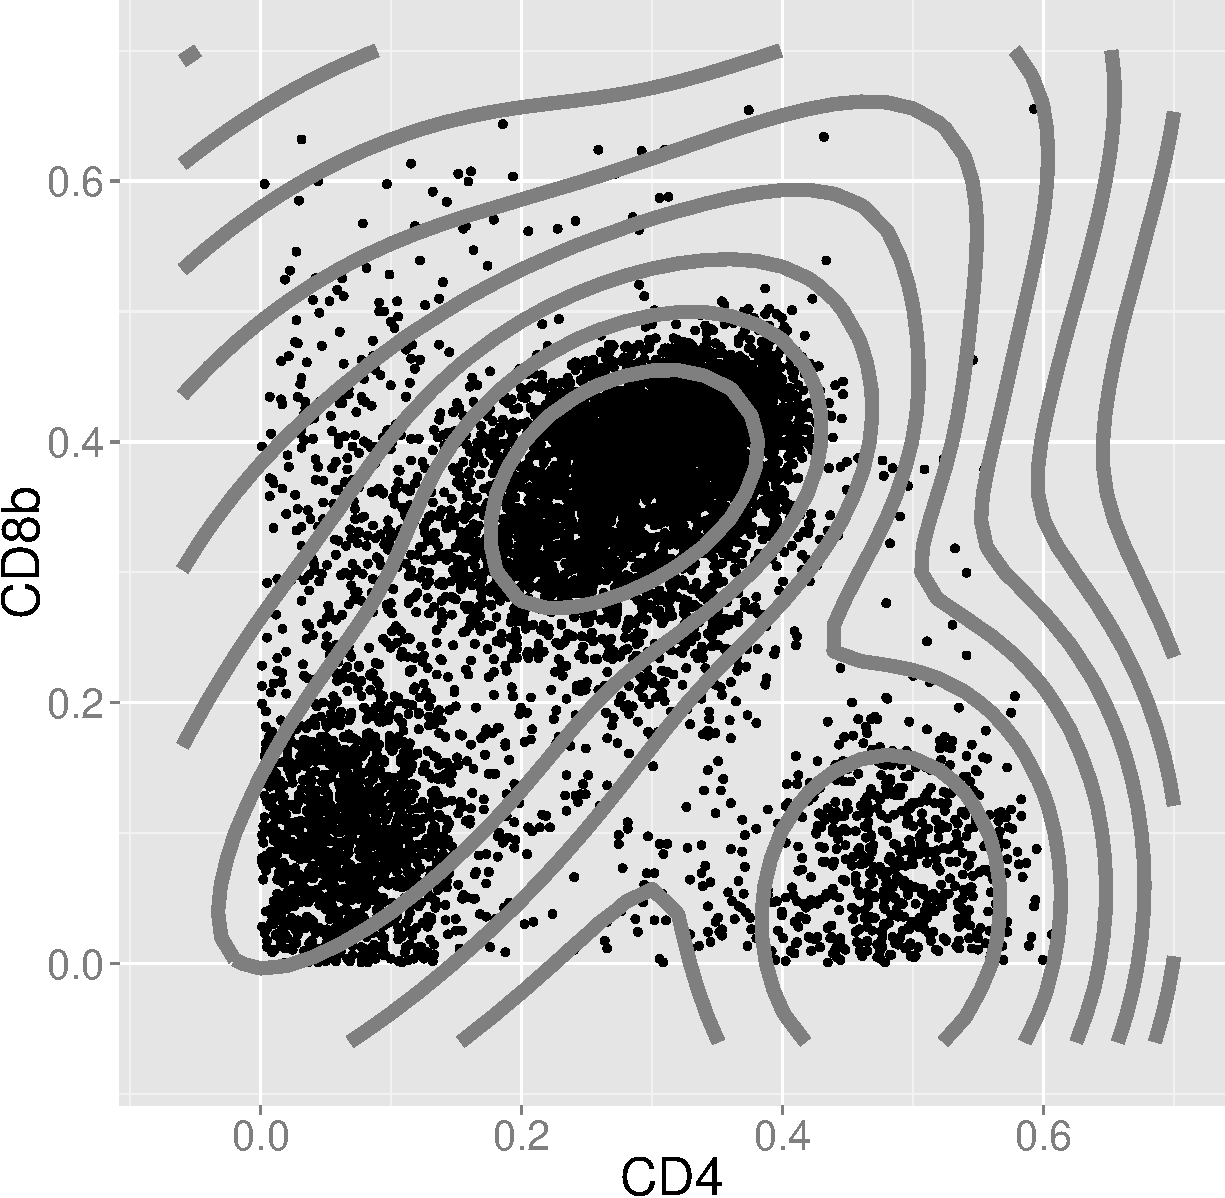
\includegraphics[width=.27\textwidth]{figs/gvhd_control.pdf}
    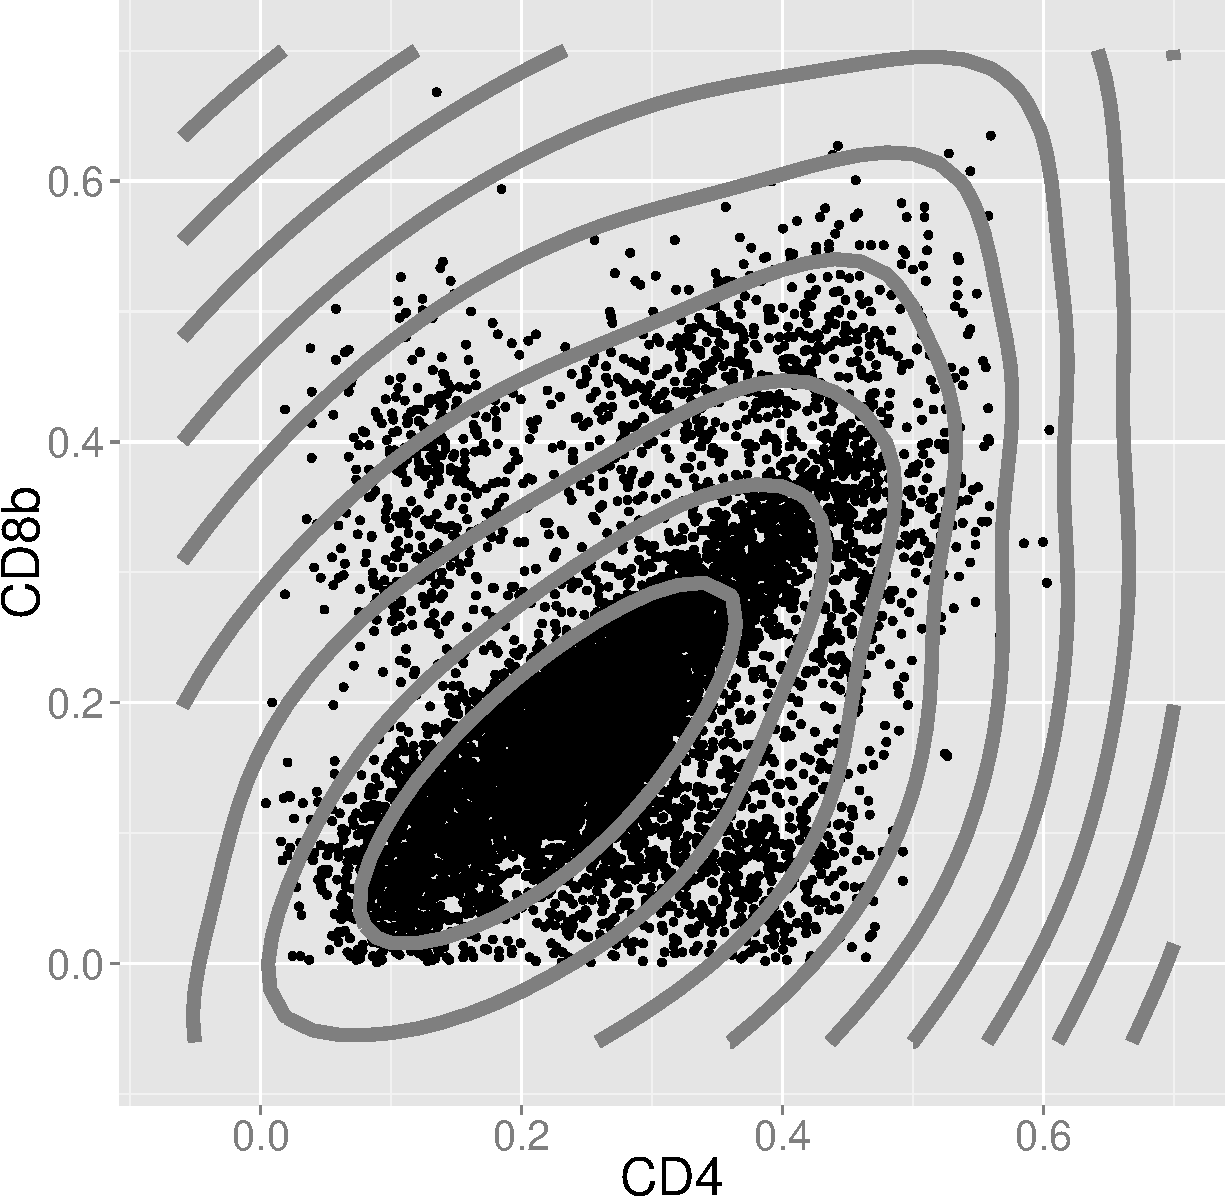
\includegraphics[width=.27\textwidth]{figs/gvhd_pos.pdf}
\caption{ Scatterplots of first two dimensions for control (left) and positive (right) group. Contours represent
log posterior-mean densities under a Dirichlet process mixture.}
  \label{fig:plot_gvhd}
  \end{figure}

We apply our algorithm to a dataset of flow cytometry measurements from patients subjected to bone-marrow transplant~\citep{Brink07}. This graft-versus-host disease
dataset has 6,809 control and 9,083 positive observations, corresponding to whether donor immune cells attack host cells.
Each observation consists of four biomarker measurements truncated between 0 and 1,024, though more complicated truncation rules are often 
used according to operator judgement~\citep{Lee2012}. We normalize and plot the first two dimensions, markers CD4 and CD8b, in 
Figure \ref{fig:plot_gvhd}.
Truncation complicates the clustering of observations into homogeneous groups, an important step in the flow-cytometry pipeline called
gating.
Consequently,~\cite{Lee2012} propose an expectation-maximization algorithm for truncated Gaussian mixture models, which must be adapted if
different mixture components or truncation rules are used. 

%We regard the normalized observations as the output of a rejection sampling algorithm that discards proposals outside the unit hypercube.
%After imputing these according to algorithm \ref{alg:rej_sim}, we can easily apply standard Bayesian models without worrying about 
%edge effects and missing probability.
We model the untruncated distribution for each group as a Dirichlet process mixture of Gaussian kernels~\citep{Lo1984}, with points
outside the four-dimensional unit hypercube discarded to form the normalized dataset.
The Dirichlet process mixture model is a flexible nonparametric prior over densities %that bypasses model selection issues like
%choosing the number of components in a Gaussian mixture model, and is 
parametrized by a concentration parameter $\alpha$ and a base probability measure.
We set $\alpha = 1$, and for the base measure, which gives the distribution over cluster parameters, we use a normal-inverse-Wishart distribution. 
%There exist standard techniques to both sample new data points for a Dirichlet process mixture, as well as to sample parameters given the augmented 
%data.
Given the rejected variables, we can use standard techniques to update a representation of the Dirichlet process. 
We follow the blocked-sampler of~\cite{IshJam2001} based on the stick-breaking representation of the Dirichlet process, using a truncation level of 
50 clusters. 
This corresponds to updating $\theta$, step 2 in Algorithm~\ref{alg:rej_post}. 
Having done this, we discard the old rejected samples, and produce a new set by drawing from a 50-component Gaussian mixture 
model, corresponding to step 1 in Algorithm~\ref{alg:rej_post}.

Figure~\ref{fig:plot_gvhd} shows the log mean posterior densities for the first two dimensions from 10,000 iterations. %Control vs Pos.
While the control group has three clear modes, these are much less pronounced in the positive group.
Directly modeling observations with a Gaussian mixture model obscured this by forcing modes away from the edges. 
One can use components with bounded support in the mixture model, such as a Dirichlet process mixture of Beta densities; however, these do not reflect the 
underlying data generation process, and are unsuitable when different groups have different
truncation levels. By contrast, it is easy to extend our modeling ideas to allow groups to share
%components \citep{TehJorBea2006}, thereby allowing better identification of disease predictors.
components, allowing better identification of disease predictors.

Our sampler took less than two minutes to run 1,000 iterations, not much longer than a typical Dirichlet process sampler for 
datasets of this size. The average number of augmented points was 3,960 and 4,608 for the two groups. We study our  sampler more systematically 
in the next section, but this application demonstrates the flexibility and simplicity of our main idea.

%this can easily be extended to identify shared clusters among the two groups \cite{Teh2006}.




\section{Bayesian inference for the matrix Langevin distribution} \label{sec:Bays_inf}

\subsection{The matrix Langevin distribution on the Stiefel manifold} \label{sec:stief_intr}
The Stiefel manifold $V_{p,d}$ is the space of all $d \times p$ orthonormal matrices, %(i.e.\ all $p$-frames in $\mathbb{R}^d$).
that is, $d \times p$ matrices $X$ such that $X^TX=I_p$, where $I_p$ is the $p \times p$  identity matrix.
%\begin{equation}
%V_{p,d}=\{X\in M(d,p): X^TX=I_p\}. \nonumber
%\end{equation}
When $p=1$, this is the $d-1$ hypersphere $S^{d-1}$, and when $p=d$, this is the space of all orthonormal matrices
$O(d)$.
Probability distributions on the Stiefel manifold play an important role in statistics, signal processing and machine learning, with applications ranging 
from studies of orientations of orbits of comets and asteroids to principal components analysis to the estimation of rotation matrices.  
%\subsection{The matrix Langevin distribution}  \label{sec:param}
The simplest such distribution is the matrix Langevin distribution,
%A random variable $X \in V_{p,d}$ distributed according to this 
an exponential-family distribution whose density with respect to the invariant Haar
volume measure~\citep{Edelman98thegeometry} is
%\begin{equation}
%\label{eq-paraML}
$\ml(X\mid F)=\etr(F^TX)/Z(F)$. %  \qquad  X \in V_{p,d}.$ %\nonumber
%\end{equation}
Here $\etr$ is the exponential-trace, and $F$ is a $d\times p$ matrix. The normalization constant $Z(F)=\mathstrut_0F_1(d/2, F^TF/4)$  is the hypergeometric
function  with matrix arguments, evaluated at $F^TF/4$~\citep{chikusebook}.
Let $F = G \bkappa H^T$ be the singular value decomposition of $F$, where $G$ and $H$ are $d \times p$ and $p \times p$ orthonormal matrices, and $\bkappa$ is
a positive diagonal matrix. 
We parametrize $\ml$ by $(G, \bkappa, H)$, and one can think of $G$ and $H$ as orientations, with $\bkappa$ controlling the
concentration in directions determined by these orientations.
%Since $F^TF = \bkappa \bkappa$, the normalization constant depends only on $\bkappa$,
Large values of $\bkappa$ imply concentration along the associated directions, while setting $\bkappa$ to zero gives the uniform distribution on
the Stiefel manifold. It can be shown~\citep{khatri1977} that $\mathstrut_0F_1(d/2, F^TF/4) =  \mathstrut_0F_1(d/2, \bkappa^T\bkappa/4)$, so that
this depends only on $\bkappa$. We write it as $Z(\bkappa$).
%with inferences carried out based on the resulting posterior. 
In our Bayesian analysis, we place independent priors on 
$\bkappa, G$ and $H$.
The last two lie on the Stiefel manifolds $V_{p,d}$ and $V_{p,p}$, and we place matrix Langevin priors $\ml(\cdot\mid F_0)$ and $\ml(\cdot\mid F_1)$ on 
these: we will see below that these are conditionally conjugate. %resulting in simple posterior update rules for these matrices.
We place independent {Gamma} priors on the diagonal elements of $\bkappa$. %writing $\kappa_i$ for element $(i,i)$ of $\bkappa$.
%  X_i      &\sim {\ml}(X_i|G\bkappa H^T)& \quad \text{for $i = 1,\ldots, n$.   \nonumber }
However, the difficulty in evaluating the normalization constant $Z(\bkappa)$ 
makes posterior inference for $\bkappa$ doubly intractable.  Thus, in a 2006 University of Iowa PhD thesis, Camano-Garcia %\cite{camanothesis} 
keeps $\bkappa$ constant, while~\cite{hoff2009jrssb} uses a first-order Taylor expansion of the intractable term to run an approximate sampling algorithm.
Below, we show how fully Bayesian inference can be carried out for this quantity as well.

\subsection{A rejection  sampling algorithm} \label{sec:prior_sim}
We first describe a rejection sampling algorithm from~\cite{hoff2009} to sample from $\ml$.
%For parameterizations other than the uniform distribution (i.e.\ for $\bkappa > 0$), even this is non-trivial.
For simplicity, assume $H$ is the identity matrix. In the general case, we simply rotate  the resulting draw 
by $H$, since if $X \sim \ml(\cdot\mid F)$, then $XH \sim \ml(\cdot\mid FH^T)$.
At a high level, the algorithm sequentially proposes vectors
from the matrix Langevin on the unit sphere: this is also called the von Mises--Fisher distribution and is easy to simulate~\citep{wood1994}.
The mean of the $r${th} vector is column $r$ of $G$, $G_{[:r]}$, projected onto the nullspace of the earlier vectors, $N_r$.
This sampled vector is then projected back onto $N_r$ and normalized, and %giving a unit vector orthogonal to the earlier $r-1$ vectors.
the process is repeated $p$ times. Call the resulting
distribution $\seq$; for more details, see Algorithm \ref{alg:rej_smplr} and~\cite{hoff2009}.
{
\vspace{.1in}
\begin{algo}{Proposal $\seq(\cdot\mid G, \bkappa)$ for the matrix Langevin distribution~\citep{hoff2009}}\label{alg:rej_smplr}
  \begin{itemize}
    \item[]
\begin{tabular}{p{.9cm}p{12.2cm}}
%\hline
{Input:}  & Parameters $G,\bkappa$; write $G_{[:i]}$ for column $i$ of $G$, and $\kappa_i$ for element $(i,i)$ of $\bkappa$. \\
{Output:} & An output  $X \in V_{p,d}$; write $X_{[:i]}$ for column $i$ of $X$. \\
\end{tabular}
\begin{tabbing}
  \enspace Sample $X_{[:1]} \sim \ml(\cdot\mid \kappa_1 G_{[:1]})$. \\
  \enspace For $r \in \{2,\cdots p\}$\\
    \qquad Construct $N_r$, an orthogonal basis for the nullspace of $\{X_{[:1]},\cdots X_{[:r-1]} \}$.\\
    \qquad Sample $z \sim \ml(\cdot\mid \kappa_r N^T_r G_{[:r]})$. \\
    \qquad Set $X_{[:r]} = z^T N_r/ \|z^T N_r\|. $
\end{tabbing}
  \end{itemize}
\end{algo}
}
Letting $I_k(\cdot)$ be the modified Bessel function of the first kind,
$\seq$ is a density on the Stiefel manifold with
\begin{align}
  \seq(X\mid G, \bkappa) &= \left\{\prod_{r=1}^p \frac{ \|\kappa_r N^T_r G_{[:r]}/2 \|^{(d-r-1)/2 }}{ \Gamma(\frac{d-r+1}{2} ) I_{(d-r-1)/2}(\| \kappa_r N^T_r G_{[:r]} \|)} \right\} \etr(\bkappa G^T X).
  %\nonumber \\ %\label{eq:hoff_seq}\\
%               &:= \etr(\bkappa G^T X)/D(X, \bkappa, G) \nonumber
\end{align}
{Write $D(X, \bkappa, G)$ for the reciprocal of the term in braces. Since
$I_k(x)/x^k$ is an increasing function of $x$, and  $\|N^T_r G_{[:r]}\| \le \|G_{[:r]}\| = 1$, we have the following bound $D(\bkappa)$ for $D(X, \bkappa, G)$:}
\begin{align}
 D(X,\bkappa, G) &\le \prod_{r=1}^p  \frac{ \Gamma(\frac{d-r+1}{2} ) I_{(d-r-1)/2}(\| \kappa_r \|)}{ \|\kappa_r/2 \|^{(d-r-1)/2 }} = D(\bkappa).\qquad \qquad \qquad \nonumber
\end{align}
This implies that $\etr(\bkappa G^T X) \le D(\bkappa) \seq(X\mid G,\bkappa) $, allowing
the following rejection sampler: sample $X$ from $\seq(\cdot)$, and accept with probability
$D(X, \bkappa, G)/D(\bkappa)$. The accepted proposals come from $\ml(\cdot\mid G,\bkappa)$, and for samples from $\ml(\cdot\mid G,\bkappa,H)$,
post multiply these by $H$.
\begin{comment}
While this approach to sampling from the prior is typically adequate, we obtain a different upper envelope to the Matrix Langevin distribution using results
from~\citep{Luke1972}.  In that work, two bounds were provided, both ideal for our purposes:
\begin{align}
  \frac{\Gamma(\nu+1)I_{\nu}(x)}{(x/2)^{\nu}} &\le e^x \left( \frac{1}{2\nu + 3} + \frac{2(\nu+1)}{2\nu+3}\left[1 + \frac{2\nu+3)x}{2(\nu+1)}\right]^{-1} \right)\quad x\ge0,\ \nu \ge -1/2,\\
  \frac{\Gamma(\nu+1)I_{\nu}(x)}{(x/2)^{\nu}} &\le \cosh(x) \quad x\ge0,\ \nu \ge -1/2
\end{align}
While, the latter is a bit more convenient, the former is tighter, and we shall use it in the following (referring to it as $b_{\nu}(x)$). For equation \eqref{eq:hoff_seq},
we have the following bound $B(X)$ on $K(X)$:
\begin{align}
 K(X) \le \prod_{r=1}^p  b_{d-r-1}(N^T_r F_{[,r]}) := B(X)
\end{align}
Now, a proposal from $\seq$ is acccepted with probability $K(X)/B(X)$.
By allowing the bound to depend on $X$, we can control the discrepancy between $B(X)$ and $K(X)$ resulting in fewer rejected samples, and greater efficiency.
Note though that our bound $B(X)$ is not uniformly tighter that the bound $B_u$ of~\citep{hoff2009}; in particular at the point $X = H$ on the Stiefel manifold,
$B(X) > K(X) = B_u$. On the other hand, our bound has the property that $\inf_{X \in V_{p,d}} K(X)/B(X) > \inf_{X \in V_{p,d}} K(X)/B_u$. This latter property will
be crucial for efficient posterior sampling. Of course, one can always combine the two bounds, defining $\hat{B}(X) = \min (B_u, B(X))$.
%is useful in its own right, providing a more efficient way to sample from the Matrix Langevin. Additionally, our approach will prove crucial for one of our
%algorithms for posterior sampling; with the bound of \cite{hoff2009} being too loose to be practical.
\end{comment}

\subsection{Posterior sampling}   \label{sec:post_sim}

Given a set of $n$ observations $\{X_i\}$, and writing $S = \sum_{i=1}^n X_i$, we have: 
\begin{align}
  p(G, \bkappa, H \mid X_i\}) & \propto {\etr(H \bkappa G^T S)p(H) p(G) p(\bkappa)}/{Z(\bkappa)^{n}}. \nonumber
\end{align}


%Recall that the normalization constant is rotation invariant (and thus independent of $H$).
At a high level, our approach is a Gibbs sampler that sequentially updates $H, G$ and $\bkappa$. %As described below, 
The pair of matrices $(H,G)$ correspond to the tractable $\theta_1$ in Algorithm~\ref{alg:rej_post}, while $\bkappa$ corresponds to $\theta_2$.
Updating the first two is straightforward, while the third requires our augmentation scheme. \\
\hspace{.1in}\\
\noindent {1. Updating $G$ and $H$:} \label{sec:update_conj} 
%The posterior distribution of $H$ is given by
%\begin{align}
%  p(H\mid X_i\},\bkappa, G) &= p(H\mid S, \bkappa, G) \propto \etr(H\bkappa G^T S)p(H).
{With a matrix Langevin prior on $H$, the posterior is }
\begin{align}
  p(H\mid X_i,\bkappa, G) & \propto \etr\left\{(S^T G \bkappa + F_0)^T H\right\}. \nonumber
\end{align}
This is just the matrix Langevin distribution over rotation matrices, and one can sample from this following Section \ref{sec:prior_sim}.
From here onwards, we will rotate the observations by $H$, allowing us to ignore this term. Redefining $S$ as $SH$, the posterior over $G$ is also
matrix Langevin,
%the conditional posterior of $G$ is given by:
\begin{align}
  p(G\mid X_i\},\bkappa) & \propto \etr\left\{(S \bkappa + F_1)^T G\right\}. \nonumber
\end{align}

\noindent {2. Updating $\bkappa$:} 
%By itself, this step intractable, since it involves
%evaluating the normalization constant $Z(\bkappa)$. % a hypergeometric function of matrix argument. % is intractable.
Here, we exploit the rejection sampler scheme of the previous section, %any observation on the Stiefel manifold is preceded by a set (possibly of size zero)
and instantiate the rejected proposals using Algorithm \ref{alg:rej_sim}. 
%A simple idea is to first conditionally sample this set of rejected proposals, and \emph{then} propose
%Let $\cY = \{Y_1,\cdots, Y_r\}$  be the sequence of $r \ge 0$ rejected proposals preceding an observation.
From Section \ref{sec:prior_sim}, the joint probability is %of the entire set is %of accepted and rejected proposals is
\begin{align}
  p(\{X_i, \cY_i\}\mid G,\bkappa)    %&  = \left( \prod_{i=1}^{|\cY|}\frac{\etr(\bkappa G^TY_i)}{D(Y_i, G, \bkappa)} \left(1 - \frac{D(Y_i, G, \bkappa)}{D(\bkappa)} \right) \right)
               %\frac{\etr(\bkappa G^TX)}{D(X, G, \bkappa)}\frac{D({X}, G, \bkappa)}{D(\bkappa)} \nonumber \\
%        &= \left( \prod_{i=1}^{|\cY|}\frac{\etr(\bkappa G^TY_i)}{D(Y_i, G, \bkappa)} \left(1 - \frac{D(Y_i, G, \bkappa)}{D(\bkappa)} \right) \right)
%              \frac{\etr(\bkappa G^T{X})}{D(\bkappa)}  \\
         &= \frac{ \etr\left\{\bkappa G^T\left(S+\sum_{j=1}^{|\cY_i|}  Y_{ij}\right ) \right\} }{D(\bkappa)^{1+|\cY|}}
             \prod_{i=1}^n   \prod_{j=1}^{|\cY|} \frac{ \left\{D(\bkappa) -  D(Y_{ij}, G, \bkappa)\right\}}{D(Y_{ij}, G, \bkappa)}.  \label{eq:rej_joint1}
\end{align}
All terms in equation~\eqref{eq:rej_joint1} can be evaluated easily, allowing %us to calculate the acceptance probability of 
a simple Metropolis--Hastings algorithm in this augmented space.
%
In fact, we can calculate gradients to run a Hamiltonian Monte Carlo algorithm~\citep{Neal2010} 
that makes significantly more efficient proposals than a random-walk sampling algorithm. %We demonstrate this below.
In particular,
%Given $n$ observations $X_1,\cdots,X_n$ with latent variable sets $\cY_1, \cdots, \cY_n$, 
let $N = n + \sum_{i=1}^n |\mathcal{Y}_i|$, and
$S = \sum_{i=1}^n(X_i + \sum_{j=1}^{|\mathcal{Y}_i|} Y_{ij})$. The log joint probability $L \equiv \log\left\{p(\{X_i,\cY_i\})\right\}$ is
\begin{align}
 L &= \text{trace}(G^T \bkappa S) +\sum_{i=1}^n \sum_{j=1}^{|\cY_i|}\left[ \log \left\{D(\bkappa) - D(Y_{ij}, \bkappa) \right\}\right. 
                        - \left. \log D(Y_{ij}, \bkappa)\right] - n \log\left\{D(\bkappa)\right. \nonumber
%\left(\sum_{i=1}^n X_i + \sum_{j=1}^{|\cY_i|}Y_{i,j} \right)
\end{align}
%Writing $D(Y, \bkappa) =
% \left\{C\prod_{r=1}^p \frac{ I_{(d-r-1)/2}(\| \kappa_r N^T_r G_r \|)}{ \|\kappa_r N^T_r G_r \|^{(d-r-1)/2 }} \right\}$ as $C\tD(Y, \bkappa) $, 
In Appendix \ref{sec:gradient}, we give an expression for the gradient of this log-likelihood. % shows that %and that $\frac{\dif }{\dif x}(x^{-m} I_m(x)) = x^{-m}I_{m+1}(x)$, we have
%
We use this to construct a Hamiltonian Monte Carlo sampler~\citep{Neal2010} for $\bkappa$. %that explores $\bkappa$-space.
Here, it suffices to note that a proposal involves taking $L$ 
leapfrog steps of size $\epsilon$ along the gradient, and accepting the resulting state with probability proportional to the product of equation
\eqref{eq:rej_joint1}, and a simple Gaussian momentum term. The acceptance probability depends on how well the
$\epsilon$-discretization approximates the continuous dynamics of the system, and choosing a small $\epsilon$ and a large $L$ can give global moves with high
acceptance probability. A large $L$ however costs a large number of gradient evaluations. We study this trade-off
in Section \ref{sec:Bayes_expt}. %, before performing a Bayesian analysis of  some problems with the Matrix Langevin distribution.
%I_d(z)/z^d$, and $D'(z) = I_{d+1}(z)/z^{d+1}$




%\section{Experiments}  \label{sec:Bayes_expt}

\subsection{Vectorcardiogram dataset}  \label{sec:vcg_np}

The vectorcardiogram is a loop traced by the {cardiac vector} during a cycle of the heart beat. The two directions of orientation of this
loop in three dimensions form a point on the Stiefel manifold. The dataset of~\cite{vecdata} includes $98$ such recordings,
and is displayed in the left panel of Figure \ref{fig:vcg_data}. We represent each observation with a pair of orthonormal vectors, with the cone of 
lines to the right forming
the first component. This empirical distribution 
possesses a single mode, so that
the matrix Langevin distribution seems a suitable model.
  \begin{figure}
  \centering
  \begin{minipage}{0.5\textwidth}
    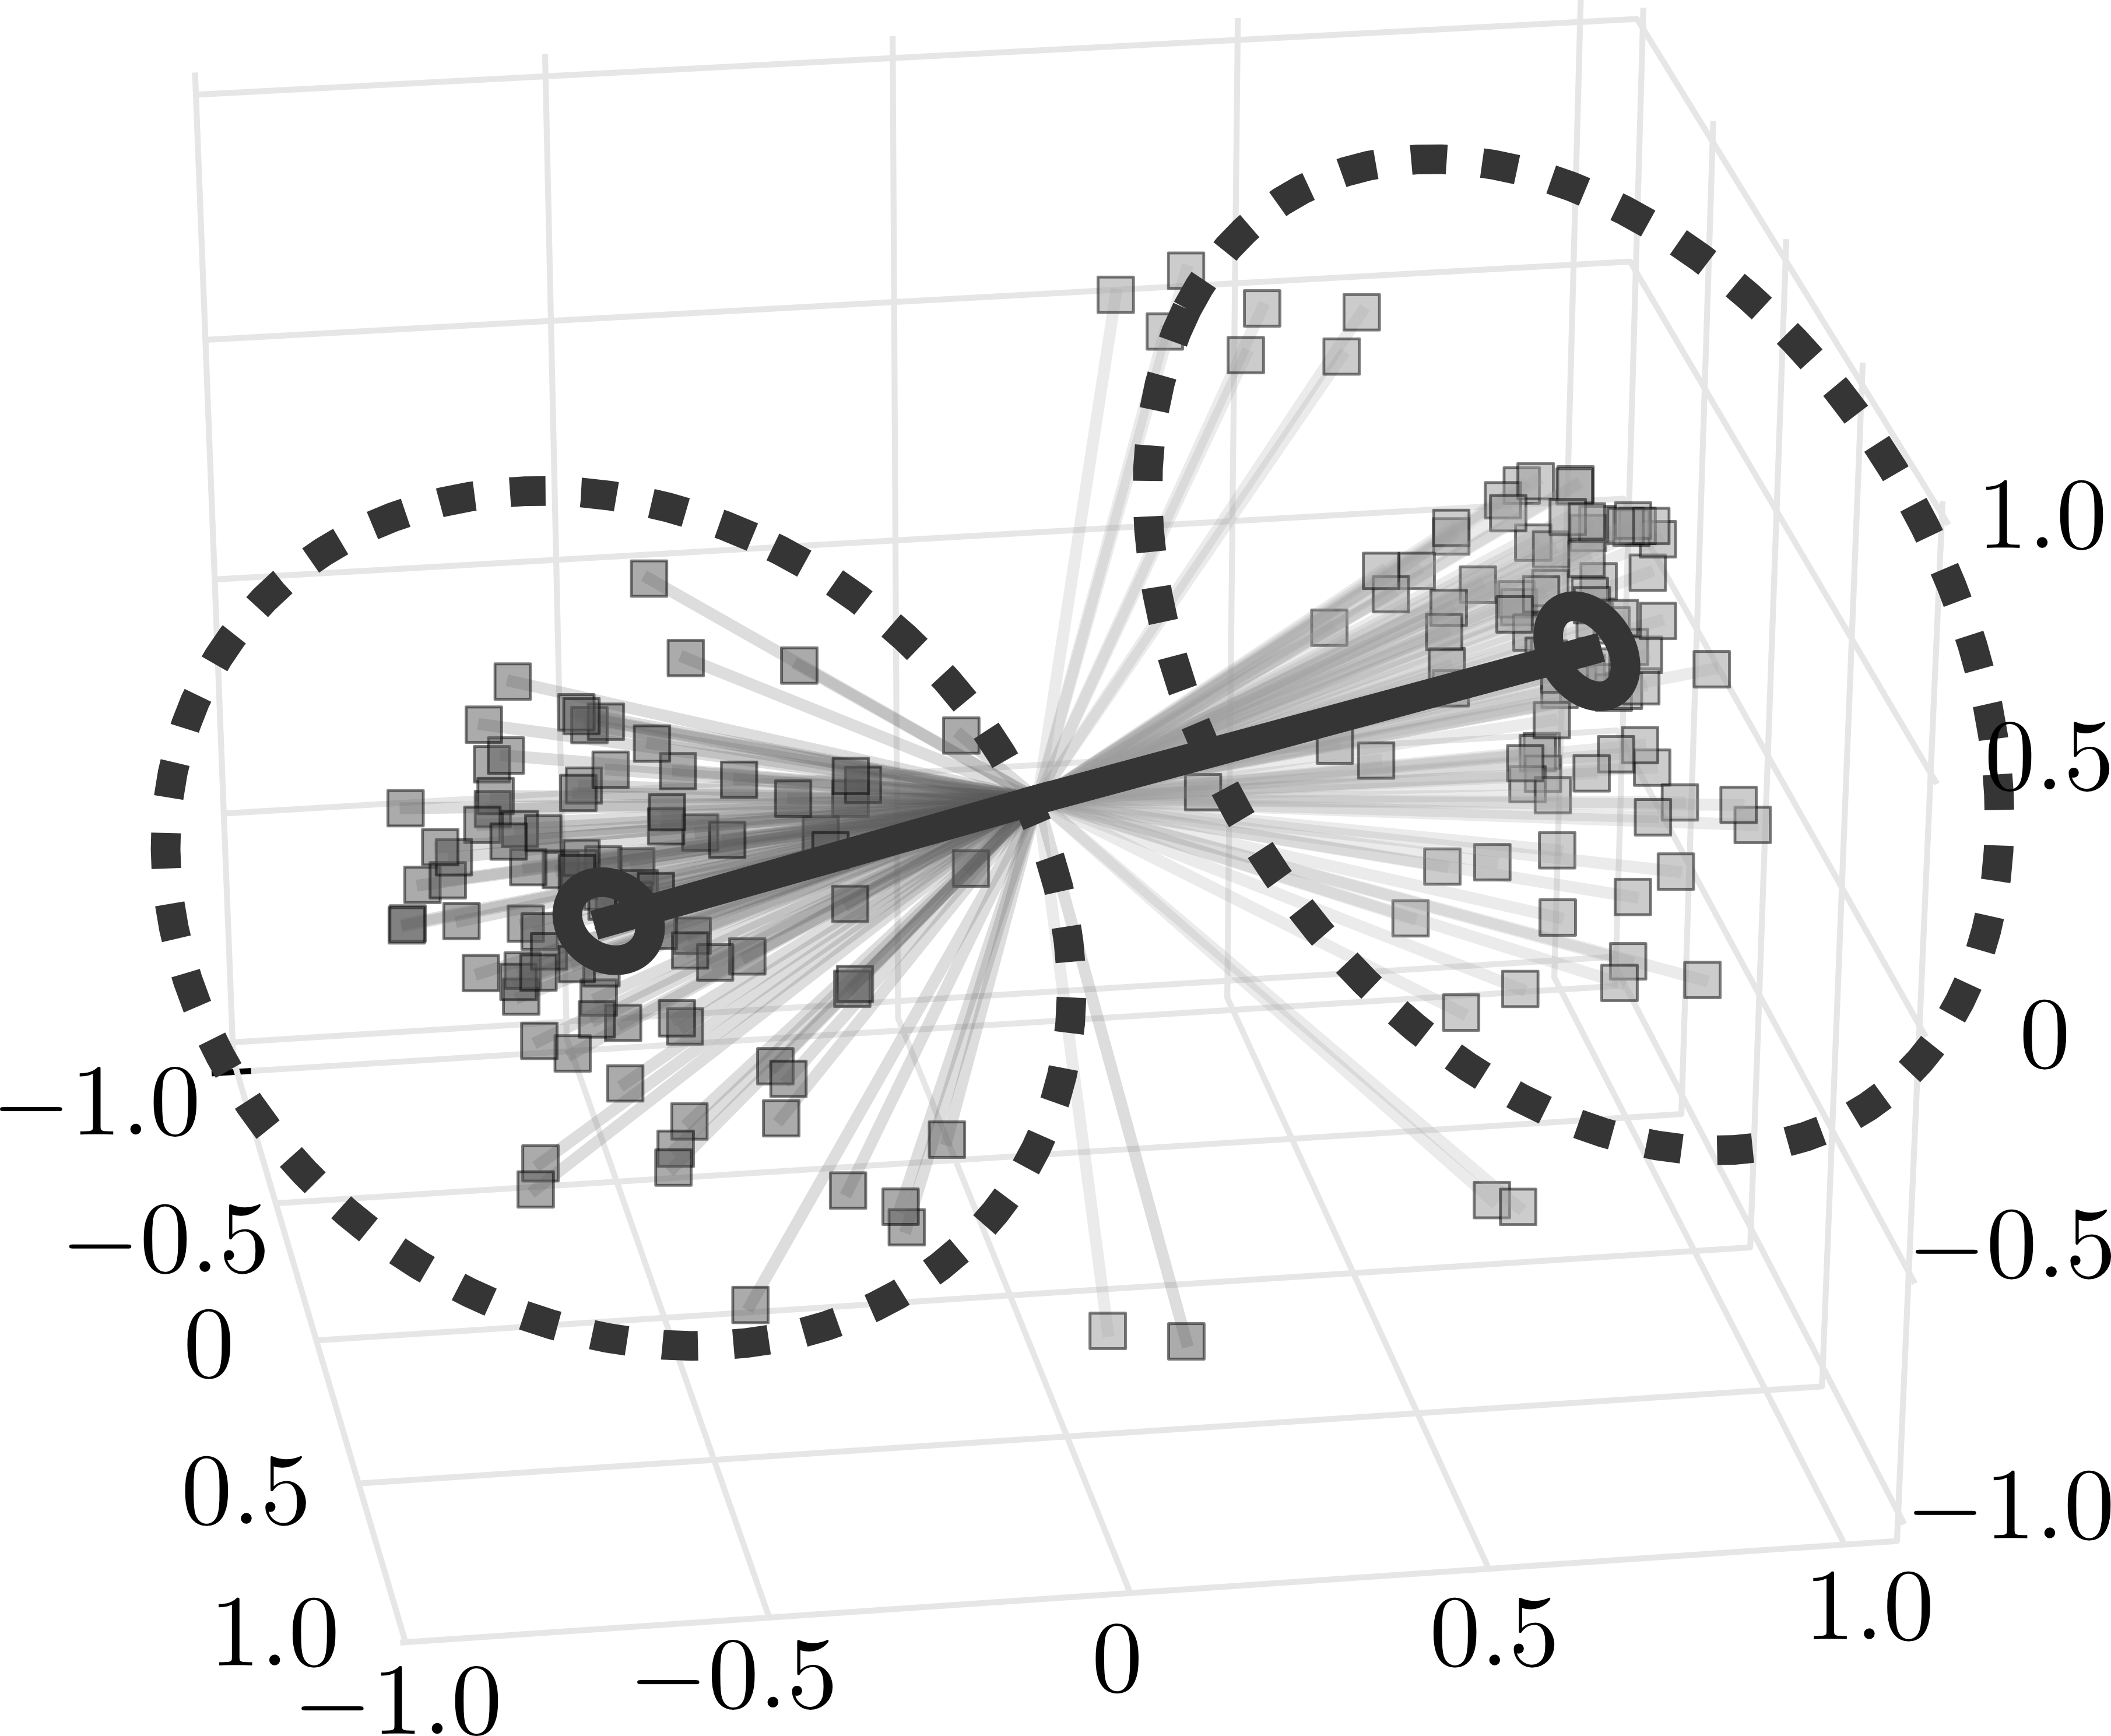
\includegraphics{figs/plot_vcg_post_bw2.png}
  \end{minipage}
  \begin{minipage}{0.4\textwidth}
  \centering
    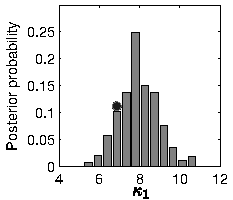
\includegraphics{figs/plot_vcg_kap1_bw.pdf}
  \centering
    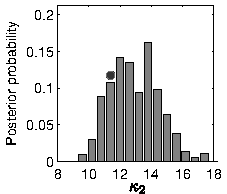
\includegraphics{figs/plot_vcg_kap2_bw.pdf}
  \end{minipage}
\caption{(Left) Vector cardiogram dataset with inferences. Bold solid lines are maximum likelihood estimates of $G$, and solid circles
 contain $90\%$ posterior mass. Dashed circles are $90\%$ predictive probability regions.
 (Right) Posterior distribution over $\kappa_1$ and $\kappa_2$, circles are maximum likelihood estimates.}
  \label{fig:vcg_data}
  \end{figure}

We place independent exponential priors with mean 10 and variance 100 on the scale parameter $\bkappa$, and a uniform prior on the location
parameter $G$. We restrict $H$ to be the identity matrix. Inferences were carried out using the Hamiltonian sampler to produce 10,000 samples, with a
burn-in period of 1,000. For the leapfrog dynamics, we set a step size of $0.3$, with the number of steps equal to 5.
We fix the mass parameter to the identity matrix.
We implemented all algorithms in $\mathtt{R}$, building on
the $\mathtt{rstiefel}$ package of~\cite{hoff2009}. 
Simulations were run on an Intel Core 2 Duo 3 Ghz CPU.
%The right plot in Figure \ref{fig:vcg_param1} shows the posterior distribution over the first component of $\bkappa$, which is centered around $1.75$
%(the second component is similar).
For comparison, we include the maximum likelihood estimates of $\bkappa$ and $G$. %; see the appendix for more details on this.
For  $\kappa_1$ and $\kappa_2$, these were $11.9$ and $5.9$, and we plot these in the right half of Figure \ref{fig:vcg_data}
as circles. 

%The blue bars show the
%Bayesian posteriors over the components of $G$.
The bold straight lines in Figure \ref{fig:vcg_data}, left, show the maximum likelihood estimates of the components of $G$, with the small
circles corresponding to $90\%$ Bayesian credible regions
estimated from the Monte Carlo output.
The dashed circles correspond to $90\%$ predictive probability regions for the Bayesian model. For these, we generated  $50$ points on $V_{3,2}$ for 
each sample, with parameters specified by that sample. The dashed circles contain $90\%$ of these points across all samples.
Figure \ref{fig:vcg_data}, right, shows the posterior over $\kappa_1$ and $\kappa_2$.

\subsection{Comparison of exact samplers} \label{sec:Bayes_expt}

%Here, we compare our sampler with the exchange sampler
%for the matrix Langevin distribution.
%the exchange sampler and our sampler based on the rejection sampler underlying the Matrix Langevin distribution.
To quantify sampler efficiency, % we explore parameter space, 
we estimate the
effective sample sizes produced per unit time. This corrects for
correlation between successive Markov chain samples
by estimating the number of independent samples produced; for this
we used the $\mathtt{rcoda}$ package of~\cite{Rcoda2006}.
%We evaluate these on the vectorcardiogram dataset.

  \begin{figure}
  \centering
    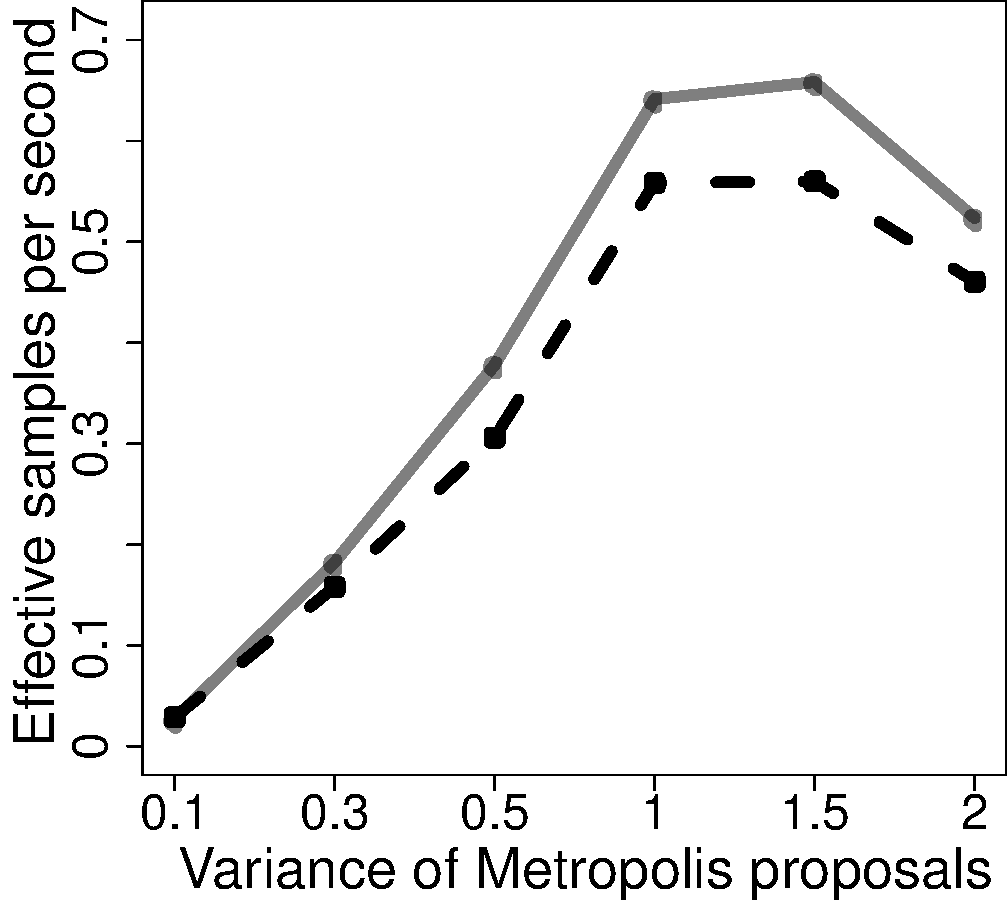
\includegraphics[width=.3\textwidth]{figs/mh_plot_bw.pdf}
  \centering
    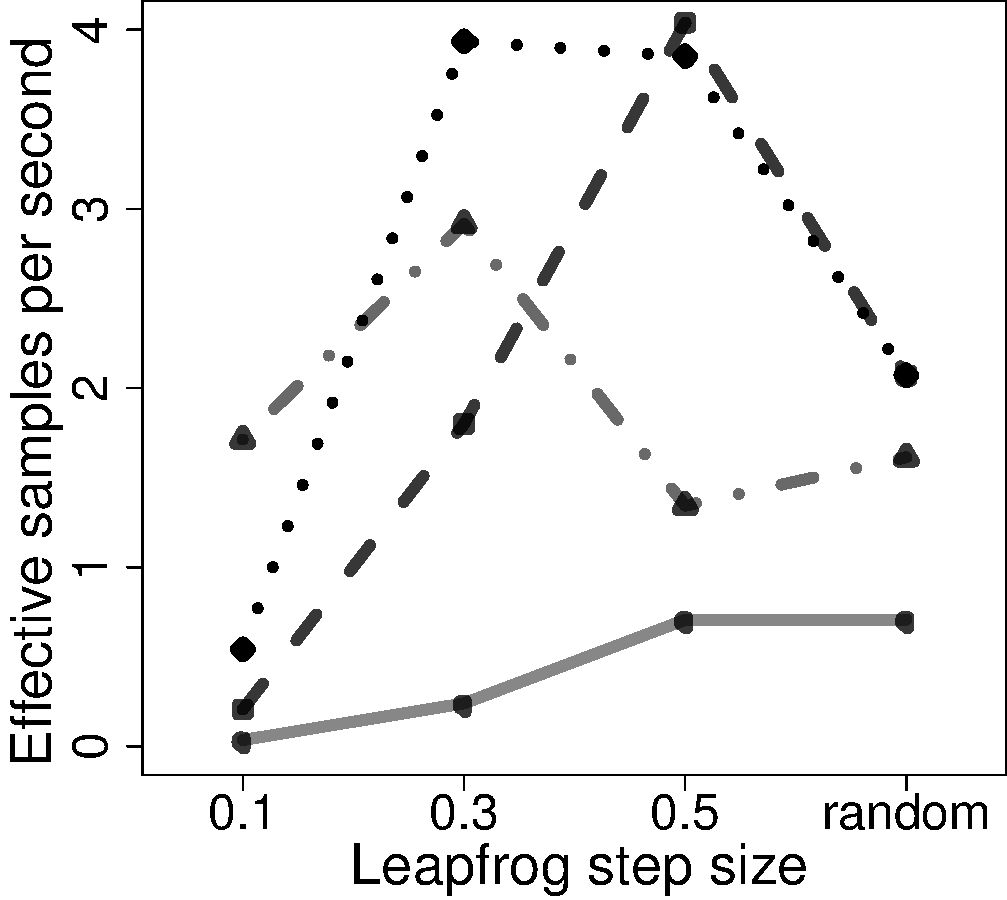
\includegraphics[width=.3\textwidth]{figs/hmc_plot_bw.pdf}
\caption{Effective samples per second for (left) random walk and (right) Hamiltonian samplers. From bottom to top at abscissa $0.5$: (left) 
 Metropolis--Hastings data-augmentation sampler and exchange sampler, and 
 (right) 1, 10, 5 and 3 leapfrog steps of the Hamiltonian sampler.}
  \label{fig:samplers_comp}
  \end{figure}

The left panel in Figure \ref{fig:samplers_comp} shows the effective sample size per second for two
Metropolis--Hastings samplers, the exchange sampler and our latent variable sampler on the vectorcardiogram dataset.
% based on
%the rejection sampler of \cite{hoff2009}. % underlying the Matrix Langevin distribution.
Both 
perform a random walk in the $\bkappa$-space, with the steps drawn for a normal
distribution whose variance increases along the horizontal axis.
%The vertical axis shows the
%median effective sample size per second for the components of $\bkappa$.
The figure shows that both samplers' performance
peaks when the proposals have a variance between $1$ and $1.5$, with the
exchange sampler performing slightly better. However, 
the real advantage of our sampler is that introducing the latent variables
results in a joint distribution with no intractable terms,
allowing the use of more sophisticated sampling algorithms. The right panel studies the Hamiltonian
Monte Carlo sampler described at the end of Section \ref{sec:latent_hist}. Here we
vary the size of the leapfrog steps along the horizontal axis, with the different
curves corresponding to different numbers of such steps.
This performs an order of magnitude better than either of the previous
algorithms, with performance peaking with $3$ to $5$ steps of size $0.3$ to
$0.5$, fairly typical values for this algorithm. This shows the advantage of exploiting
gradient information in exploring the parameter space.


\subsection{Comparison with an approximate sampler}
In this section, we consider an approximate sampler based on an asymptotic approximation to 
$Z(\bkappa)= \mathstrut_0F_1(d/2, \bkappa^T\bkappa/4)$ for large values of
$(\kappa_1, \ldots, \kappa_n)$~\citep{khatri1977}:
\begin{align}
  Z(\bkappa)  \simeq &
         \left\{ \frac{2^{-\frac{1}{4}p(p+5) + \frac{1}{2}pd}}{\pi^{\frac{1}{2}p}} \right\} \etr(\bkappa) \prod_{j=1}^p \Gamma\left(\frac{d-j+1}{2} \right)
   \left[ \left\{\prod_{j=2}^p \prod_{i=1}^{j-1}(\kappa_i + \kappa_j)^{\frac{1}{2}} \right\} \prod_{i=1}^p \kappa_i^{\frac{1}{2}(d-p)} \right]^{-1}. \nonumber
\end{align}
%An expansion, similar in spirit, but for the matrix Bingham distribution was used by \cite{hoff2009jrssb}. 
We use this approximation in the acceptance probability
of a Metropolis--Hastings algorithm; it can similarly be used to construct a Hamiltonian sampler. 
For a more complicated but accurate approximation, see~\cite{Kume:2013:SAN}. In general however, using
such approximate schemes involves the ratio of two approximations, and can
have very unpredictable performance. %Below, we study the behaviour of this approximation along with the performance of our exact sampler.
  \begin{figure}
  \centering
    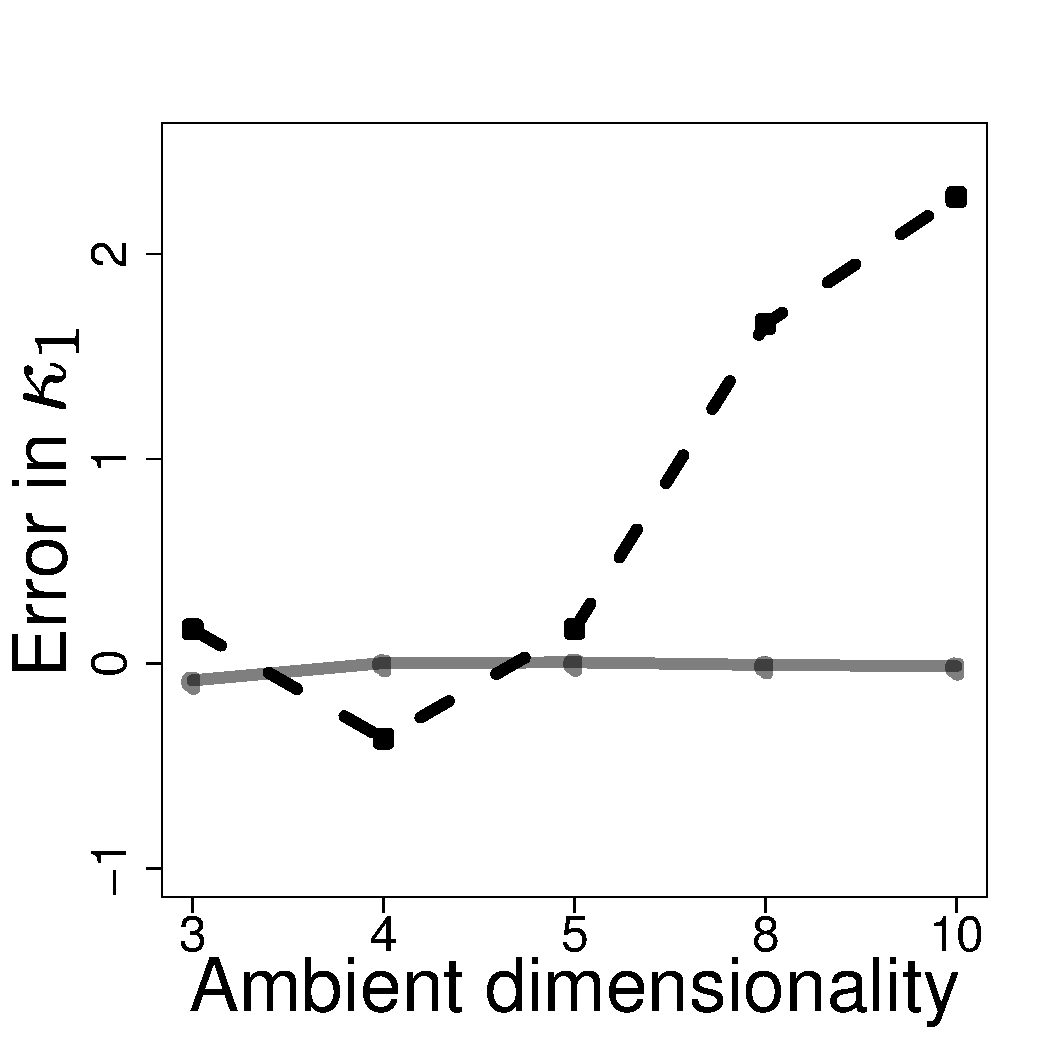
\includegraphics[width=.25\textwidth]{figs/approx_err1_bw.pdf}
  \centering
    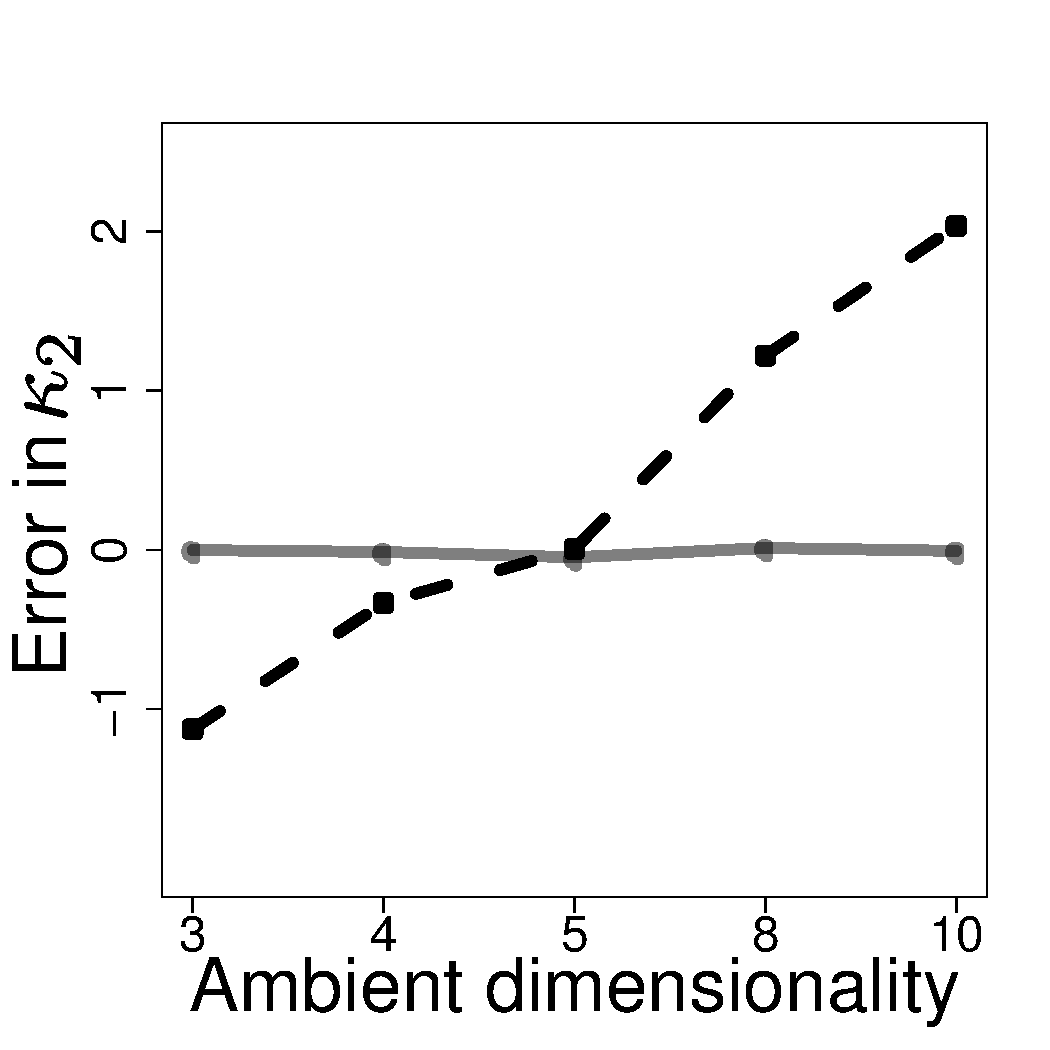
\includegraphics[width=.25\textwidth]{figs/approx_err2_bw.pdf}
  \centering
    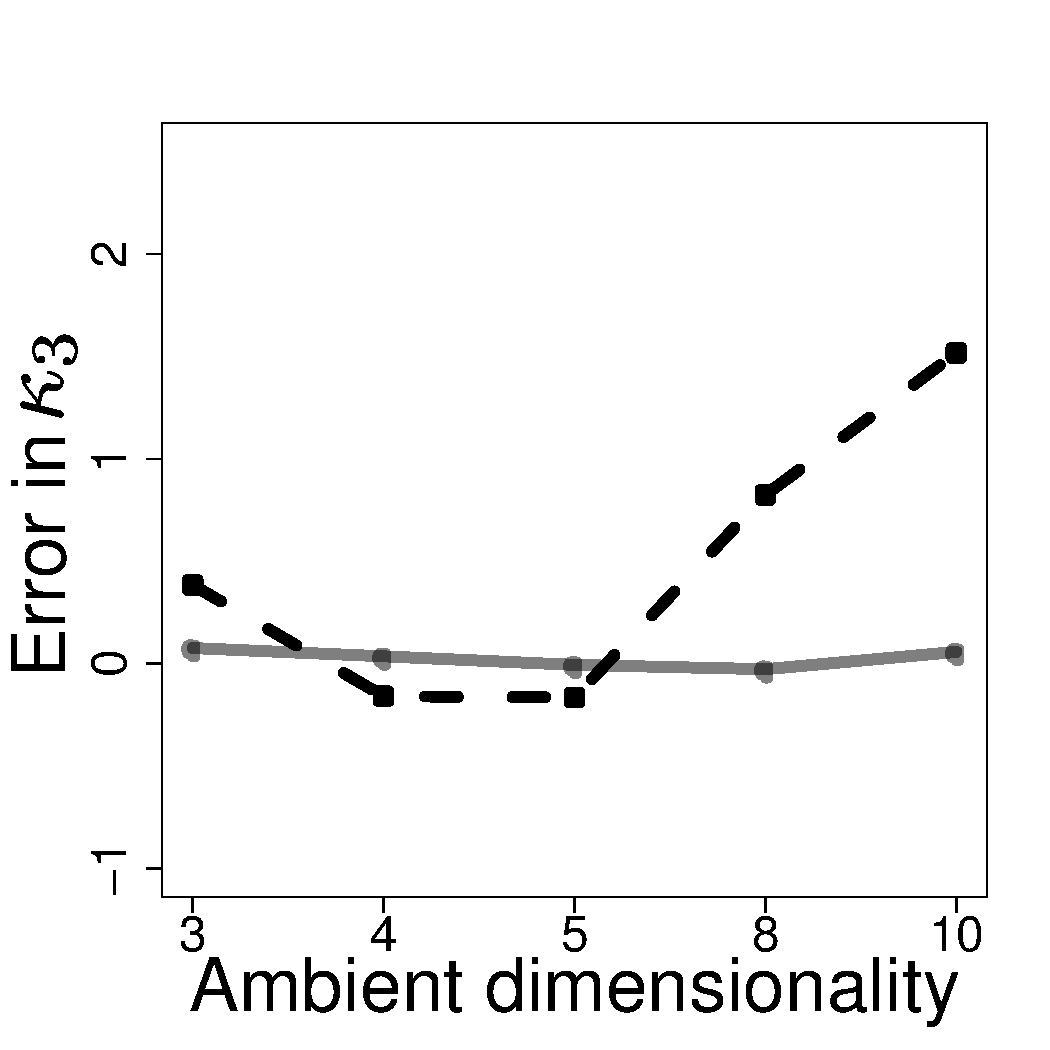
\includegraphics[width=.25\textwidth]{figs/approx_err3_bw.pdf}
\caption{Errors in the posterior mean for the vectorcardiogram
dataset. Each panel is a different component of $\kappa$; solid/dashed lines are the Hamiltonian/approximate sampler.}
  \label{fig:approx_comp}
  \end{figure}

On the vectorcardiogram dataset, the approximate sampler 
is about forty times faster than the exact samplers. For larger
datasets, this difference will be even greater, and the real question is how accurate
the approximation is. Our exact sampler allows us to study this: %we consider different values of $\bkappa$ and 
%different dimensions of the ambient space. In particular, 
we consider the Stiefel manifold $V_{d,3}$,
with the three diagonal elements of $\bkappa$ set to $1, 5 $ and $10$. With this setting of $\bkappa$, and
a random $G$, we generate datasets with $50$ observations, with $d$ taking values $3, 4, 5, 8,$ and $10$.
In each case, we estimate the posterior mean of $\bkappa$ by running the exchange sampler, and treat this as the
truth. We compare this with posterior means returned by our Hamiltonian sampler, as well as the approximate sampler.  Figure \ref{fig:approx_comp}
shows these results. 
%with the three subplots corresponding to the three components of $\bkappa$, and ambient dimensionality
%$d$ increasing along the horizontal axis.
As expected, the two exact samplers agree, and the Hamiltonian sampler has almost no error.
%The approximate sampler is more complicated. 
For values of $d$ around $5$, the estimated posterior mean for the approximate sampler is close to that of the exact samplers. Smaller values lead to an approximate posterior mean that underestimates the actual posterior mean,
while in higher dimensions, the opposite occurs. Recalling that $\bkappa$ controls the concentration of the matrix Langevin distribution about its
mode, this implies that in high dimensions, the approximate sampler underestimates uncertainty in the distribution of future observations.


\section{The Gaussian process density sampler}\label{sec:gpds}
\subsection{Nonparametric density modeling with a transformed Gaussian process}
Our next application is the Gaussian process density sampler of~\cite{adams_gpds},
%This finds application in Bayesian density modeling applications, where one wishes to place 
a nonparametric prior for probability densities induced by a logistic transformation of a random function from a Gaussian process.  
Letting $\sigma(\cdot)$ denote the logistic function, the random density is 
%$$p(x) \propto g(x) \sigma\{ f(x) \},\quad 
%f \sim \mbox{\small{GP}}, $$
\begin{align}
g(x) &\propto g_0(x) \sigma\{f(x)\},\qquad
f \sim  \mbox{\small{GP}}, \nonumber 
\end{align}
with $g_0(\cdot)$ a parametric base density and $\mbox{\small{GP}}$ denoting a Gaussian process.
%However, %the fact that the sigmoid is bounded above by $1$ gives us 
The inequality
%\begin{align}
$g_0(x) \sigma\{f(x)\} \le g_0(x)$
%\end{align}
allows a rejection sampling algorithm %where we draw perfect samples by successively 
by making proposals from $g_0(\cdot)$.
%can do this sequentially, sampling a new 
At a proposed location $x^*$, we sample the function value $f(x^*)$ conditioning on 
all previous evaluations, and accept the proposal with probability 
$\sigma\{f(x^*)\}$.  Such a scheme involves no approximation error, and only requires evaluating the random function on a finite set of points.
Algorithm \ref{alg:gpds} describes the steps involved in generating $n$ observations.

{
\begin{algo}
{Generate $n$ new samples from the Gaussian process density sampler}\label{alg:gpds}
\begin{itemize}
  \item[]
\begin{tabular}{p{.9cm}p{12.2cm}}
{Input:}  & A base probability density $g_0(\cdot)$. \\
                 & Previous accepted and rejected proposals $\tilde{X}$ and $\tilde{Y}$. \\
                 & Gaussian process evaluations $f_{\tilde{X}}$ and $f_{\tilde{Y}}$ at these locations. \\
{Output:} & $n$ new samples $X$, with the associated rejected proposals $Y$. \\ % from the random density $p(\cdot)$.  \\
                 & Gaussian process evaluations $f_X$ and $f_Y$ at these locations. \\
\end{tabular}
\vspace*{-8pt}
\begin{tabbing}
  \enspace Repeat \\
  \qquad Sample a proposal $y$ from $g_0(\cdot)$. \\
  \qquad Sample $f_y$, the Gaussian process evaluated at $y$, conditioning on $f_X$, $f_Y$, $f_{\tilde{X}}$ and $f_{\tilde{Y}}$. \\ % at $X$ and $Y$  %, and the covariance kernel $\mathcal{K}$.
  \qquad {With probability }{$\sigma(f_y)$} \\
  \qquad \qquad Accept $y$ and add it to $X$. Add $f_y$ to $f_X$.\\
  \qquad  {Else} \\
  \qquad  \qquad Reject $y$ and add it to $Y$. Add $f_y$ to $f_Y$.\\
  \enspace Until {$n$ samples are accepted}.
\end{tabbing}
\end{itemize}
\end{algo}
}



\subsection{Posterior inference}
% The GPDS defines a nonparametric prior over probability densities on $\mathbb{X}$. 
Given observations $X = \{x_1, \ldots, x_n\}$,
we are interested in $p(g\mid X)$, the posterior over the underlying density. %, or equivalently, % $p(\cdot)$. 
Since $g$ is determined by the modulating function $f$, we focus on %there is a one-to-one mapping between the density and the 
%function $f(\cdot)$, we focus on 
$p(f\mid X)$. %By itself, this is a complicated quantity, and 
While this quantity is doubly intractable,
after augmenting the state space to include the proposals $\cY$ from the rejection sampling algorithm, %of the previous section results in a much simpler probability distribution. 
%In particular, 
 $p(f\mid X,\cY)$ has density $\prod_{i=1}^n \sigma\left\{f(x_i)\right\} \prod_{i=1}^{|\cY|} \left[1-\sigma\left\{f(y_i)\right\}\right]$
  with respect to the Gaussian process prior; see also~\cite{adams_gpds}.
In words, the posterior over $f$ evaluated at $X \cup \cY$ is just the posterior from a Gaussian process
classification problem with a logistic link-function, and with the accepted and rejected proposals corresponding to the two classes.
%x_i &\sim p(x) \qquad i = 1, \cdots, n
Markov chain Monte Carlo methods such as Hamiltonian Monte Carlo or elliptical slice sampling~\citep{murray2010} 
are applicable in such a situation. Given $f$ on $X \cup \cY$, the Gaussian process can be evaluated anywhere else by 
conditionally sampling from a multivariate normal.

%The question then is how to 
Sampling the rejected proposals $\cY$ given $X$ and $f$ is straightforward by Algorithm \ref{prop:rej_post}:
run the rejection sampler until $n$ accepts, and treat the rejected proposals generated
along the way as $\cY$. In practice, we do not have access to the entire function $f$, only its
values evaluated on $X$ and $\cY_{old}$, the locations of the previous thinned variables. However, just as under the generative 
mechanism, we can retrospectively evaluate the function $f$ where needed.
After proposing from $g_0(\cdot)$, we sample the value of the function at this location conditioned on all previous evaluations, and
use this value to decide whether to accept or reject. We outline the inference algorithm in
Algorithm \ref{alg:gpds_mcmc}, noting that it is much simpler than that proposed in~\cite{adams_gpds}.
We also refer to that paper for limitations of the exchange sampler in this problem.

  \begin{figure}
  \centering
    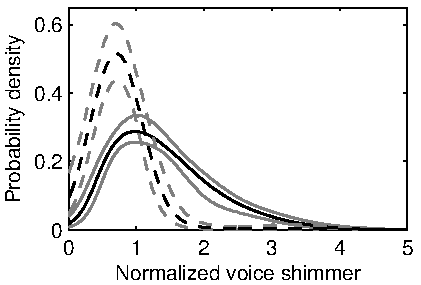
\includegraphics[width=.35\textwidth]{figs/plot_parkinson_new.pdf}
    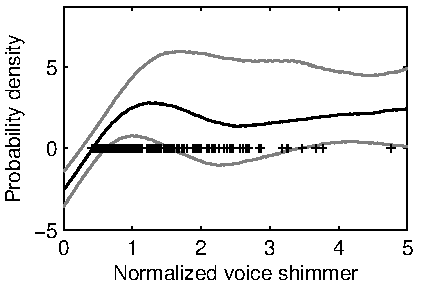
\includegraphics[width=.35\textwidth]{figs/plot_parkinson_int_new.pdf}
\caption{Inferences for the Parkinson's dataset: (left) posterior density for positive/control groups, shown as 
solid/ dashed lines, (right) posterior distribution of the Gaussian process function for
positive group with observations. Both panels show the median with $80$ percent credible intervals.}
  \label{fig:plot_glx}
  \end{figure}
{
\begin{algo}{A Markov chain iteration for inference in the Gaussian process density sampler}\label{alg:gpds_mcmc}
  \begin{itemize}
    \item[]
\begin{tabular}{p{.9cm}p{12.2cm}}
{Input:}  & Observations $X$ with corresponding function evaluations $\tilde{f}_X$. \\
          & Current rejected proposals $\tilde{Y}$ with corresponding function evaluations $\tilde{f}_{\tilde{Y}}$. \\
{Output:} & New rejected proposals $Y$. \\ % from the random density $p(\cdot)$.  \\
                 & New Gaussian process evaluations $f_X$ and $f_Y$ at $X$ and $Y$. \\
                 & New hyperparameters. \\
\end{tabular}
\begin{tabbing}
  \enspace Run Algorithm \ref{alg:gpds} to produce $|X|$ accepted samples, with $X, \tilde{Y}, \tilde{f}_X$ and $\tilde{f}_{\tilde{Y}}$ as inputs. \\
  \enspace Replace $\tilde{Y}$ and $f_{\tilde{Y}}$ with values returned by the previous step; call these $Y$ and $\hat{f}_Y$.\\
  \enspace Update $\tilde{f}_X$ and $\hat{f}_Y$ using for example, hybrid Monte Carlo, to get $f_X$ and $f_Y$.\\
  \enspace Update Gaussian process and base-distribution hyperparameters.
\end{tabbing}
  \end{itemize}
\end{algo}
}


\subsection{Experiments}   \label{sec:gpds_expt}

  Voice changes are a symptom and measure of onset of Parkinson's disease, and one attribute is voice shimmer, a measure of variation in
  amplitude. We consider a dataset of such measurements for subjects with and without the disease~\citep{little07}, with
%Voice-shimmer is a measure of variation in amplitude, and there are 
147 measurements with, and 48 without the disease.
We normalized these to vary from $0$ to $5$, and  used the model of~\cite{adams_gpds} as a prior on the underlying probability densities. 
We set $g_0(\cdot)$ to a normal $\mathcal{N}(\mu,\sigma^2)$, 
with a normal-inverse-Gamma prior on $(\mu, \sigma)$. The latter had its mean, inverse-scale, degrees-of-freedom and variance
set to $0,.1,1$ and $10$. The Gaussian process had a 
squared-exponential kernel, with variance and length-scale of $1$.
For each case, we ran a Matlab implementation of our data augmentation algorithm to produce 2,000 posterior samples after a burn-in of $500$ samples. 

  \begin{figure}
  \centering
    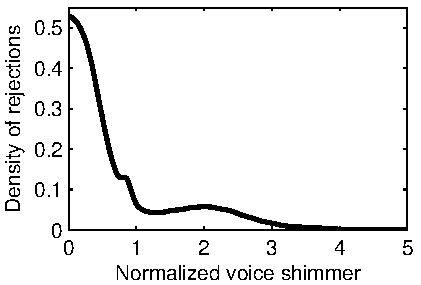
\includegraphics[width=.35\textwidth]{figs/plot_park_thin.pdf}
    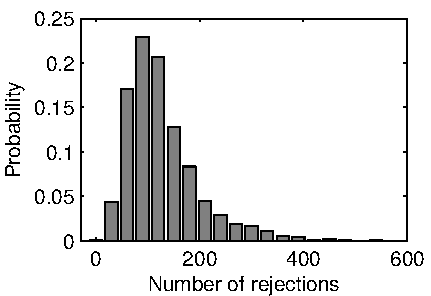
\includegraphics[width=.35\textwidth]{figs/plot_park_thin2.pdf}
\caption{Rejected proposals for the Parkinson's dataset: (left) kernel density estimate of locations of rejected proposals, and (right) histogram of 
the number of rejected proposals for the positive group.}
  \label{fig:plot_glx2}
  \end{figure}


  The left panel in Figure~\ref{fig:plot_glx} shows the resulting posterior over densities, corresponding to $\theta$ in Algorithm~\ref{alg:rej_post}.
The control group is fairly Gaussian, while the disease group is skewed to the right.
%This is clearly multimodal and non-Gaussian, with the modulating function allowing low-probability areas around either side of the main cluster
%of observations. The right bump away from the origin is slightly thinner that the left one because we have fewer observations there, but also
%since we centered our model around the origin.
The right panel focuses on the deviation from normality by plotting the posterior over the latent function $f$. 
%Outside the interval $[0,10]$, this reverts to the prior, with the decaying tails of the base-measure $g_0(\cdot)$ accounting for the lack of observations there. 
%Inside the interval $[0,10]$, there are two dips in the Gaussian process intensity at $[1,3]$
%and $[7,9]$, while over $[3,7]$, it 
We see that to the right of $0.5$, this deviation is larger than its prior mean of zero, implying larger probability than under a Gaussian density.
Figure~\ref{fig:plot_glx2} studies the distribution of the rejected proposals $\cY$.
The left plot shows the distribution of their locations:
most of these occured near the origin. Here, the disease density reverts to Gaussian or even sub-Gaussian density, with the intensity function taking small 
values.  The right plot is a histogram of the number of rejected proposals: this is typically 
around 100 to 150, though
the largest value we observed was $668$. Since inference on the latent function involves evaluating it at the accepted as
well as rejected proposals, the largest covariance matrix we had to deal with was about $600 \times 600$; typical values were around $100 \times 100$. Using
the same setup as Section~\ref{sec:Bayes_expt}, it took a na\"ive Matlab implementation 26 and 18 minutes to run 2,500 iterations for the
disease and control datasets. One can imagine 
computations becoming unwieldy for a large number of observations, or when there is large mismatch between the true density and the base-measure $g_0(\cdot)$. 
In such situations, one might have to choose the Gaussian process covariance kernel more carefully, use one of many sparse approximation techniques,
or use other nonparametric priors like splines instead. In all these cases, we can use our algorithm to recover the rejected proposals $\cY$, 
and given these, posterior inference for $f$ 
can be carried out using standard techniques.
%, this effect
%vanishes when we place a more uniformative prior on the parameters of $g_0(\cdot)$.




\section{Future work}\label{sec:conc}
%like Hamiltonian Monte Carlo to carry out efficient inference. 
Our algorithm, while exact, also provides a framework for faster, approximate algorithms.
A priori, the number of rejected proposals preceeding any observation is 
%a random number that a priori 
unbounded: one can bound the computational cost of an iteration by limiting the maximum number
of rejected proposals. Similarly, one might share rejected proposals across observations. We leave
the study of such approximate sampling algorithms %resulting from such user impatience 
for future research. Also left open is a more careful analysis
of Markov mixing rates for the applications we considered. There are also a
 number of applications that we have
not described here: particularly relevant are rejection samplers for 
%stochastic differential
diffusions~\citep{beskos06,bladt2014} .




\section*{Acknowledgement}
This work was supported by the National Institute of Environmental Health Sciences of the National Institute of Health.
We are grateful to the editor and reviewers for valuable comments.


\appendix
\section{Proofs}

% \begin{proof}[of Proposition \ref{prop:rej_post}]

% The probability density of an accepted sample $x$ is
% $p(x\mid \theta) = {f(x,\theta)}/{Z(\theta)}$.
% {Independently introduce the set $(\cY, \hat{x})$ by running the rejection sampler until acceptance, so that}
% \begin{align}
%   p(x, \cY, \hat{x}\mid \theta) &=\frac{f(x,\theta)}{Z(\theta)}
%                      \left[ \frac{f(\hat{x}, \theta)}{M} \prod_{i=1}^{|\mathcal{Y}|}  \left\{q(y_i\mid \theta) - \frac{f(y_i, \theta)}{M}\right\} \right]  \nonumber \\
%             &=\frac{f(\hat{x},\theta)}{Z(\theta)}
%                      \left[\frac{f({x}, \theta)}{M} \prod_{i=1}^{|\mathcal{Y}|}  \left\{(q(y_i\mid \theta) - \frac{f(y_i, \theta)}{M}\right\} \right]. \nonumber
% \end{align}
% {Marginalizing out $\hat{x}$, we have $
%   p(\cY, x) =  \frac{f(x, \theta)}{M} \prod_{i=1}^{|\mathcal{Y}|}  \left\{q(y_i\mid \theta) - \frac{f(y_i, \theta)}{M} \right\}$}.\\ %\nonumber
% From equation \eqref{eq:rej_jnt}, we see this is the desired joint distribution, proving our scheme is correct.
% \end{proof}

\begin{proof}[of Proposition~\ref{prop:rej_post}]
  Rejection sampling first proposes from $q(x|\theta)$, and then accepts with probability $f(x,\theta)/\{Mq(x|\theta)\}$. %or rejects them.
  Conceptually, one can first decide whether to accept or reject, and then conditionally sample the location.
  The marginal acceptance probability is $Z(\theta)/M$, the area under $f(\cdot,\theta)$ divided by that under $M q(\cdot\mid\theta)$.
  An accepted sample $x$ is distributed as the target distribution $f(x, \theta)/Z(\theta)$, while rejected samples are distributed as 
  $\left\{{Mq(x\mid\theta) - f(x,\theta)}\right\}/\left\{M-Z(\theta)\right\}$. This two-component mixture is just the proposal $q(x)$.
  While this mixture representation loses the computational benefits of the original algorithm, it shows that the location of an accepted sample is independent
  of the past, and consequently, that the number and locations of rejected samples preceding an accepted sample is independent of the location
  of that sample. Thus, one can use the rejected samples preceding any other accepted sample.
\end{proof}




\begin{proof}[of Theorem~\ref{thrm:conv_rate}]
It follows from Bayes' rule and the assumed bounds that for an observation $X$,
    $$p(\theta\mid X,\cY) \ge p(\theta\mid X) \frac{b_f}{B_f} \left(\frac{b_qr}{B_q}\right)^{|\cY|}.$$
 Let the number of observations $|X|$ be $n$. Then,
\begin{align}
  k(\htheta\mid \theta) &= \int_{\bU^n} p(\htheta\mid \cY,X) p(\cY\mid \theta,X) \mathrm{d}\cY \nonumber \\
  & \ge  \left(\frac{b_f}{B_f}\right)^n p(\htheta\mid X) \prod_{i=1}^n \int_{\bU} \beta^{|\cY_i|} p(\cY_i\mid \theta,X)  \mathrm{d}\cY_i \nonumber \\
    & =  \left(\frac{b_f}{B_f}\right)^n p(\htheta\mid X) \prod_{i=1}^n \int_{\bU} \beta^{|\cY_i|}  \frac{Z(\theta)}{M}  \prod_{j=1}^{|\cY_i|}  \left\{q(y_{ji}\mid \theta) - \frac{ f(y_{ji}, \theta)}{M} \right\} \lambda(\mathrm{d}y_{ji}) \nonumber \\
    & =  \left\{\frac{b_f Z(\theta)}{B_f M}\right\}^n{p(\htheta\mid X)} 
    \prod_{i=1}^n \sum_{|\cY_i| = 0}^{\infty} \beta^{|\cY_i|}  \prod_{j=1}^{|\cY_i|}  \left\{1 - \frac{Z(\theta)}{M} \right\} \nonumber \\
%    & =  \frac{p(\htheta|X)}{M^n} \prod_{i=1}^n \sum_{|\cY_i| = 0}^{\infty} \beta^{|\cY_i|}  \left(1 - \frac{1}{M} \right)^{|\cY_i|} \nonumber  \\
%    & =  {p(\htheta\mid X)} \left\{\frac{b_f Z(\theta)}{B_f M}\right\}^n\prod_{i=1}^n \frac{1}{\tilde{\delta}_{\theta}}, \qquad \tilde{\delta}_{\theta} = 1 - \beta\left\{1-Z(\theta)/M\right\} \nonumber \\
& =  {p(\htheta\mid X)} \left\{\frac{b_f Z(\theta)}{B_f M}\right\}^n\prod_{i=1}^n \frac{1}{1 - \beta\left\{1-Z(\theta)/M\right\}} \nonumber \\
    & =   \frac{p(\htheta\mid X)}{\delta_{\theta}^n}, \qquad {\delta_{\theta}} = \frac{B_f}{b_f}\left[ \frac{M}{Z(\theta)} - \beta\left\{\frac{M}{Z(\theta)}-1\right\}\right]
    =  \frac{B_f}{b_f}\left\{ \frac{M}{Z(\theta)} (1 - \beta) + \beta\right\} \nonumber \\ %M(1-\beta) - \beta  \nonumber 
%           & \ge   {{\delta}}{p(\htheta\mid X)} \qquad \frac{1}{\delta^{\frac{1}{n}}} = \frac{B_f}{b_f}\left( \frac{1}{R} - \beta(\frac{1}{R}-1)\right)
%           =  \frac{B_f}{b_f}\left( \frac{1}{R} (1 - \beta) + \beta)\right) \nonumber \\ %M(1-\beta) - \beta  \nonumber 
& \ge   {{\delta}}{p(\htheta\mid X)}, \qquad \delta = \left\{\frac{b_f}{B_f\left( \beta + R^{-1}\right)}\right\}^n. \nonumber
\end{align}
Thus $k(\htheta\mid \theta)$ satisfies equation \eqref{eq:unif_erg}, with 
$ \delta = \left[ {b_f}\left\{{B_f\left( \beta + R^{-1}\right)}\right\}\right]^n$, and $h(\htheta) = p(\htheta\mid X)$.
\end{proof}
 \label{sec:proofs}
%\input{proofs_long.tex} 

\section{Gradient information}

For $n$ pairs $\{X_i, \cY_i\}$, %1,\ldots,X_n$ and rejections $\cY_1, \ldots, \cY_n$, 
with $\tilde{n} = n + \sum_{i=1}^n |\mathcal{Y}_i|$, and
$S = \sum_{i=1}^n(X_i + \sum_{j=1}^{|\mathcal{Y}_i|} Y_{ij})$, we have %The log joint probability is
%\begin{align}
% \log\left[p(\{X_i,\cY_i\}|\bkappa,G)\right] &= \text{trace}(G^T \bkappa S) +\sum_{i=1}^n \sum_{j=1}^{|\cY_i|}\left[ \log \left\{D(\bkappa) - D(Y_{ij}, \bkappa) \right\}\right.  %\nonumber \\
% - \left. \log\left\{D(Y_{ij}, \bkappa)\right\}\right] - \tilde{n} \log\left\{D(\bkappa)\right\}. \nonumber
%%\left(\sum_{i=1}^n X_i + \sum_{j=1}^{|\cY_i|}Y_{ij} \right)
%\end{align}
\begin{align}
  \log\left[p(\{X_i,\cY_i\}|\bkappa)\right] &= \text{trace}(\bkappa G^T S) +\sum_{i=1}^n \sum_{j=1}^{|\cY_i|} \log \left\{\frac{D(\bkappa) - D(Y_{ij}, \bkappa) }{  %\nonumber \\
  D(Y_{ij}, \bkappa)}\right\} - \tilde{n} \log D(\bkappa). \nonumber
%\left(\sum_{i=1}^n X_i + \sum_{j=1}^{|\cY_i|}Y_{ij} \right)
\end{align}
Let $\tD(Y, \bkappa) =
{\prod_{r=1}^p { \|\kappa_r N^T_r G_{[:r]} \|^{-(d-r-1)/2 }}{ I_{(d-r-1)/2}(\| \kappa_r N^T_r G_{[:r]} \|)} }$, and %, so that $D(Y,\bkappa) = C\tD(Y, \bkappa)$.
 $\tD(\bkappa) =
 {\prod_{r=1}^p { \|\kappa_r \|^{-(d-r-1)/2 }}{ I_{(d-r-1)/2}(\| \kappa_r \|)} }$.
 Since ${\dif }\left\{{x^{-m}}{I_m(x)} \right\}/{\dif x}= x^{-m}I_{m+1}(x)$, 
\begin{align}
  \quad  \frac{\dif \tD(Y, \bkappa)}{\dif \kappa_j} & = N^T_jG_{[:j]} \tD(Y,\bkappa) \frac{I_{(d-j+1)/2}}{I_{(d-j-1)/2}}(\kappa_j N^T_jG_{[:j]} ),  \quad  %\nonumber\\
\quad  \frac{\dif \tD(\bkappa)}{\dif \kappa_j}     = \tD(\bkappa) \frac{I_{(d-j+1)/2}}{I_{(d-j-1)/2}}(\kappa_j). \nonumber
\intertext{Then, writing $L = \log p(\{X_i,\cY_i\}|\bkappa) $, and $\tD'$ for $\mathrm{d}\tD/\mathrm{d}\kappa_k$, we have}
%from equation~\eqref{eq:rej_joint1}}
\frac{\dif L }{\dif \kappa_k} &= G_{[:k]}^T S_{[:k]} +\sum_{i=1}^n \sum_{j=1}^{|\cY_i|}\left\{\frac{\tD'(\bkappa) - \tD'(Y_{ij}, \bkappa) }{\tD(\bkappa) - \tD(Y_{ij}, \bkappa)} -
\frac{\tD'(Y_{ij}, \bkappa) }{\tD(Y_{ij}, \bkappa) }  \right\} - \tilde{n}\frac{\tD'(\bkappa)}{\tD(\bkappa)}  \nonumber\\
%   &=  G_{[,k]}^T S_{[,k]} +\sum_{i=1}^n \sum_{j=1}^{|\cY_i|}\left(\frac{\tD'(\bkappa)\tD(Y_{ij},\bkappa) - \tD(\bkappa)
%                            \tD'(Y_{i,j}, \bkappa) }{\tD(Y_{i,j}, \bkappa) (\tD(\bkappa) - \tD(Y_{i,j}, \bkappa))}  \right)
%              - N  \frac{I_{(d-j+1)/2}}{I_{(d-j-1)/2}}(\kappa_k)  \\
%   &=  G_{[,k]}^T S_{[,k]} +\sum_{i=1}^n \sum_{j=1}^{|\cY_i|}\left(\frac{\tD'(\bkappa) - \tD(\bkappa)N^T_kG_k \frac{I_{(d-k+1)/2}}{I_{(d-k-1)/2}}(\kappa_k N^T_kG_k ) }
%                            { (\tD(\bkappa) - \tD(Y_{i,j}, \bkappa))}  \right)  \nonumber \\
%       & \qquad       - N  \frac{I_{(d-j+1)/2}}{I_{(d-j-1)/2}}(\kappa_k)  \\
&\hspace{-.0in}=  G_{[:k]}^T S_{[:k]} +\sum_{i=1}^n \sum_{j=1}^{|\cY_i|}\left\{\frac{ \frac{I_{(d-k+1)/2}(\kappa_k)}{I_{(d-k-1)/2}(\kappa_k)}  - 
N^T_kG_{[:k]} \frac{I_{(d-k+1)/2}(\kappa_k N^T_kG_{[:k]} )}{I_{(d-k-1)/2}(\kappa_k N^T_kG_{[:k]} )} }
                             { 1 - {\tD(Y_{ij}, \bkappa)}/{\tD(\bkappa)}}  \right\}  
                             - \tilde{n}  \frac{I_{(d-k+1)/2}(\kappa_k)}{I_{(d-k-1)/2}(\kappa_k)}. \nonumber
\end{align}

 \label{sec:gradient}


\bibliographystyle{biometrika}
%\bibliographystyle{plain}
\bibliography{refs}

\end{document}
